\documentclass[10pt, a4paper]{aqademic}

\usepackage[spanish]{babel}
\selectlanguage{spanish}

\usepackage[default]{sourcesanspro}
\usepackage[T1]{fontenc}

% Document packages

\usepackage{amsmath}
\usepackage{amsfonts}
%\usepackage[type=CC, modifier=by-nc-sa, version=4.0]{doclicense}
\usepackage{graphicx}
\graphicspath{{img/}}
\usepackage[numbers]{natbib}
\usepackage{enumitem}
\usepackage{colortbl}
\usepackage{tikz}

% Document settings

\definecolor{green500}{HTML}{4caf50}
\definecolor{brown500}{HTML}{795548}

% Nest enumeration as numbers
\renewcommand{\labelenumii}{\theenumii}
\renewcommand{\theenumii}{\theenumi.\arabic{enumii}.}

\author{Juan Ocaña Valenzuela}
\title{Trabajo Fin de Grado}

\AqSetChapter{Capítulo}

% Document composition

\begin{document}

\AqMaketitle[%
	cover    = img/logo.png,
	org      = Grado en Ingeniería Informática,
	subtitle = Aplicación de gestión de rutinas semanales basada en tecnologías web
]
\tableofcontents

\listoffigures

% Capítulo: introducción
\chapter{Introducción}

\section{Resumen}
\textbf{Palabras clave:} desarrollo web, \textit{React}, \textit{Typescript}, aplicación web, \textit{REST}, arquitectura cliente-servidor

\bigskip

Existe una gran oferta en cuanto a herramientas de organización personal. Desde activas comunidades que apuestan por formatos tradicionales como agendas y calendarios personalizados hasta numerosos servicios preparados para ajustarse a cualquier tipo de persona, escoger un método de organización puede suponer una odisea para alguien interesado en la materia. 

\medskip

Muchas de las herramientas más populares en este campo optan por ofrecer un servicio de suscripción ---a menudo con versión gratuita---, que aporta ventajas tales como la sincronización de los datos del usuario en la nube o integración con servicios adicionales. Sin embargo, a veces estas opciones son demasiado complejas para algunas personas, que simplemente buscan algo más sencillo o acorde a sus necesidades.

\medskip

Se plantea una propuesta de aplicación con una funcionalidad simple, orientada a asistir en la creación de rutinas y hábitos, utilizando como soporte un sistema de objetivos y una estructura de horario semanal. La idea principal es brindar una funcionalidad simple a la vez que intuitiva, haciendo énfasis en la facilidad de uso, optando por no incluir herramientas complejas, tales como un sistema de calendario o un bloc de notas ---opciones que muchos de los servicios mencionados anteriormente implementan---.

\medskip

La aplicación propuesta se ha desarrollado utilizando tecnologías web extendidas y con gran soporte en la actualidad, y una arquitectura cliente-servidor basada en el patrón \textit{REST} \cite{fielding2000architectural}. Se ha hecho énfasis en el aprendizaje de nuevas tecnologías, como \textit{TypeScript} \cite{bierman2014understanding}, \textit{React} \cite{react} o el popular entorno de desarrollo Django \cite{django}, junto con su \textit{Django REST Framework} \cite{drf}.

\newpage


\section{\textit{Abstract}}

\textbf{Keywords:} web development, \textit{React}, \textit{Typescript}, web application, \textit{REST}, client-server architecture

\bigskip

There is a huge offer in personal organization tools. From active communities reviving and reinventing traditional methods, like journals and custom calendars, 
to numerous software services ready to accomodate to every kind of person, choosing a personal organizing system can be an epic task for any interested person.

\medskip

A lot of software resources offer a versatile and complete solution, often binded to a subscription model with a free trial. This approach offers serious advantages, like data sync between devices, or first-party support in the rest of the provider's ecosystem of tools. However, these options can be rather overwhelming for some users, who look for a simple solution fitting their everyday needs.

\medskip

The proposed application offers a simple functionality, with emphasis on creating and maintaining week-based routines, using objectives defined by the user, streaks, a registry, and a weekly timetable structure. The objective is to keep the application as easy to use as possible, without overloading it with extra functionalities that users might not need and other solutions already provide. 

\medskip

This application has been developed using modern web technologies used worldwide, using extended concepts like a component-based framework like React \cite{react},
the TypesScript language \cite{bierman2014understanding}, the popular Django Web Framework \cite{django} and its plugin \textit{REST Framework} \cite{drf}, and a client-server architecture.


\newpage

\section{Integración de conocimientos previos}

Este proyecto se centra en la adquisición de nuevos conocimientos a la hora de desarrollar aplicaciones web, así como en el desarrollo de los aquiridos a lo largo del grado. A continuación se repasan varias materias útiles en la elaboración de este trabajo, así como las asignaturas en las que se imparten y desarrollan.

\subsection*{Conocimientos de bases de datos}

Ha sido de especial utilidad conocer los diferentes tipos de sistemas gestores de bases de datos, sus ventajas e inconvenientes, y el manejo de lenguajes de 
consulta como SQL. También ha resultado indispensable el saber cómo establecer una conexión con una base de datos, realizar un correcto modelo de los mismos, 
y aprovechar el esquema relacional.

\textbf{Asignaturas útiles} 

\begin{itemize}
	\item Fundamentos de Bases de Datos
	\item Diseño y Desarrollo de Sistemas de Información
	\item Sistemas de Información Basados en Web
\end{itemize}


\subsection*{Conocimientos de desarrollo web}

Pese a haber trabajado poco en este campo anteriormente, los conocimientos previos en la materia han sido de gran ayuda de cara a comprender el funcionamiento de tecnologías como TypeScript, HTML, el protocolo HTTP o el patrón Modelo-Vista-Controlador, así como el funcionamiento de un servidor web y la infraestructura necesaria para un proyecto de estas características. Además, las prácticas de empresa realizadas en el grado han complementado la formación recibida, ya que se ha trabajado con diferentes tecnologías web.

\textbf{Asignaturas útiles}

\begin{itemize}
	\item Sistemas de Información Basados en Web
	\item Fundamentos de Redes
	\item Servidores Web de Altas Prestaciones
	\item Prácticas de empresa
\end{itemize}


\subsection*{Conocimientos de metodologías de desarrollo y gestión de proyectos}

Dado que este proyecto se centra en los aspectos del desarrollo utilizando metodologías ágiles, los conocimientos adquiridos en el grado acerca de ello han sido de vital importancia para la realización del mismo.

\textbf{Asignaturas útiles}

\begin{itemize}
	\item Fundamentos de Ingeniería del Software
	\item Metodologías de Desarrollo Ágil
	\item Dirección y Gestión de Proyectos
\end{itemize}


\begin{itemize}
	\item Fundamentos de Bases de Datos
	\item Fundamentos de Ingeniería del Software
	\item Ingeniería de Servidores
	\item Sistemas de Información Basados en Web
	\item Dirección y Gestión de Proyectos
	\item Metodologías de Desarrollo Ágil
\end{itemize}

% Capítulo: estado del arte
\chapter{Estado del arte}

\section{Crítica al estado del arte}

El mercado de aplicaciones de organización personal está repleto de opciones, con algunas de ellas muy populares. Las aplicaciones estudiadas pueden dividirse en las siguientes categorías, según su principal enfoque en cuanto a la organización personal

\subsection*{Aplicaciones de agenda y calendario}

Las aplicaciones de agenda y calendario son las más populares, debido a su enfoque principalmente profesional. Se trata de herramientas completas y potentes, con capacidad para gestionar diferentes calendarios simultáneos, recordatorios, exportación a distintos formatos e integración con otros servicios ---como por ejemplo es el caso de Google Calendar, en el que se pueden planificar citas a través de \textit{Gmail}, o adjuntar salas de videoconferencia de \textit{Google Meet}---. 

\medskip

Una de las principales ventajas de los principales servicios de este tipo es su gratuidad. Al estar mantenidos en su mayoría por grandes empresas tecnológicas ---Google, Microsoft, Apple, etc.---, no requieren de un esfuerzo adicional para el usuario del resto de sus respectivas aplicaciones.

\medskip

Estos servicios, pese a estar preparados para un uso intensivo y profesional, también se adaptan al usuario medio en mayor o menor medida. No obstante, su complejidad puede resultar abrumadora, y ante todo, suplen necesidades específicas: una agenda y un calendario tradicionales.

\medskip

Algunas de las aplicaciones de calendario más populares o influyentes son las siguientes:

\begin{itemize}
	\item Google Calendar
	\item Microsoft Outlook
	\item Apple Calendar (anteriormente llamado \textit{iCal})
\end{itemize}


\subsection*{Aplicaciones de tareas}

Otro enfoque popular a la hora de ofrecer herramientas de organización personal es el de las aplicaciones de tareas. Estos servicios ofrecen la posibilidad de planificarse a través de listas de tareas, a menudo con añadidos como notificaciones y recordatorios, similares a los presentes en las aplicaciones más tradicionales anteriormente mencionadas. 

\medskip

Estas aplicaciones utilizan la \textbf{tarea} como elemento base, construyendo todo su funcionamiento en torno a ella, y poniendo el foco en facilitar la interacción del usuario con la misma. Pese a estar presentes en entornos profesionales, muchas de estas aplicaciones se orientan hacia el usuario medio en primer lugar, ofreciendo una experiencia más sencilla e intuitiva.

\medskip

No obstante, muchos de estos servicios cuentan con una funcionalidad limitada, a menudo como expositor de una suscripción; y aquellos que no disponen de esta opción suelen requerir de un esfuerzo adicional por parte del usuario ---por ejemplo, Tasks.org \cite{tasks.org}---.

\medskip

Algunos ejemplos de aplicaciones de tareas son las siguientes:

\begin{itemize}
	\item any.do
	\item Todoist
	\item Tasks.org
\end{itemize}


\subsection*{Aplicaciones de espacio de trabajo}

Existen aplicaciones cuya premisa es ofrecer al usuario diversas herramientas para crear su método de organización, con todas las ventajas de un soporte digital. Estas aplicaciones suelen brindar al usuario sistemas de bases de datos sencillos y fáciles de manipular, con tal de organizar notas y documentos compuestos de distintos módulos preestablecidos. No existe un estándar para las aplicaciones de este tipo, y cada servicio define su propio sistema ---por ejemplo, \textit{Notion} centra sus esfuerzos en las bases de datos, mientras que \textit{Evernote} lo hace en un completo sistema de notas---.

\medskip

Pese a que este tipo de aplicaciones ofrecen una gran versatilidad, requieren un esfuerzo adicional por parte del usuario para comprender y aprender a utilizar las herramientas a su disposición. 

\medskip

Algunas aplicaciones de este tipo son las siguientes:

\begin{itemize}
	\item Notion
	\item Evernote
	\item Microsoft OneNote
\end{itemize}

\subsection*{Aplicaciones de seguimiento de hábitos}

Por último, existe una categoría de aplicaciones de organización enfocadas al seguimiento de diferentes objetivos, ya sean definidos por el usuario o preestablecidos en base a unas pautas concretas. 

\medskip

Dichas aplicaciones, mayoritariamente publicadas para dispositivos móviles, permiten registrar los avances del usuario en diferentes tareas, contabilizar el progreso y presentarlo en distintos formatos. Muchas de estas aplicaciones implementan sistemas de ludificación \cite{inproceedings} ---también llamada \textit{gamificación}---, utilizando logros, puntos y otros mecanismos similares para mantener el interés del usuario.

\medskip

Un aspecto relevante de estos servicios es que suelen centrarse en temáticas específicas, como el deporte, hábitos saludables, productividad o registro del estado de ánimo, por poner algunos ejemplos. Casi todos ellos siguen orientados a construir rutinas, ya sean diarias, como mantener un horario de sueño constante, hidratarse o regar las plantas, o con diferentes plazos ---semanales, mensuales, personalizados, etc.---, pero la forma de presentar la información al usuario es muy diferente. 

\medskip

Debido a las grandes diferencias entre las aplicaciones de seguimiento de hábitos estudiadas, es difícil definir un usuario objetivo claro. Están orientadas a un perfil personal, pero muchas de ellas tratan de implementar soluciones a problemas demasiado específicos y abusan de la ludificación, volviendo su uso tedioso.

\medskip

Algunas aplicaciones populares en este ámbito son las siguientes:

\begin{itemize}
	\item Rabit
	\item Dailyo
	\item Habit (\textit{Leap Fitness Group})
	\item Habitica
\end{itemize}


\subsection*{Crítica}

No faltan soluciones de este tipo en el mercado. Desde un ámbito más profesional hasta el usuario más ajeno a la tecnología, existe una gran variedad de aplicaciones para organizarse, con diversos enfoques y objetivos. 

Pese a lo completas y maduras que son las aplicaciones más tradicionales, su enfoque profesional y multitud de funcionalidades pueden suponer un obstáculo para un perfil de usuario que no sólo no va a beneficiarse de todas las integraciones y ventajas que ofrecen, sino que no las necesita. 

\medskip

Las aplicaciones de tareas suplen este exceso de complejidad con un planteamiento básico y suficiente, añadiendo funciones complementarias, a menudo similares a las de servicios tradicionales, pero adaptadas al flujo de la lista de tareas. No obstante, muchas de estas funciones requieren de una suscripción, estando las aplicaciones muy limitadas en su versión gratuita al no disponer de una infraestructura tan grande. 

\medskip

Las aplicaciones de espacio de trabajo son herramientas muy potentes, que en manos de usuarios experimentados pueden resultar muy útiles y servir multitud de propósitos. Muchas de ellas ofrecen plantillas predefinidas para usos comunes, y permiten establecer sistemas de organización a medida, pero suelen centrarse en colecciones de datos en lugar de eventos y tareas, y aunque puedan definirse fechas, notificaciones y, en algunos casos, calendarios, suelen ser atributos secundarios, que necesitan trabajo previo por parte del usuario para funcionar.

\medskip

Por último, las aplicaciones de seguimiento de hábitos siguen un propósito específico, alejado del resto de sistemas. Su especificidad hace que este tipo de aplicaciones sean fáciles de entender con respecto a otras soluciones. No requieren de gran configuración previa, su función es limitada pero concreta, y sirven como apoyo al usuario para conseguir sus objetivos y ver su progreso de forma sencilla, independientemente de los medios que utilicen para llevarlos a cabo. No pretenden ser un sustituto de otros servicios como las aplicaciones de calendario o espacios de trabajo, y pueden llegar a complementarse muy bien.

No obstante, pese a que gozan de gran popularidad y variedad, muchas de ellas ofrecen incentivos y mecanismos tan distintos al usuario que pueden resultar desde poco interesantes a abrumadoras. Además, el soporte de muchas de estas aplicaciones comparadas con el resto de casos estudiados suele ser escaso, o depender de servicios externos a configurar por el usuario. Esto último no es necesariamente algo negativo, pero puede inclinar al usuario a explorar otras opciones.


\section{Propuesta}

Debido a la gran variedad y flexibilidad que se puede encontrar en el mercado, las aplicaciones de seguimiento de hábitos son un marco perfecto para desarrollar un proyecto utilizando tecnologías web: presenta una variedad de requisitos aceptable, un modelo de datos interesante, y peticiones específicas de un posible cliente que se han de satisfacer. Además, una aplicación de este estilo puede beneficiarse del formato propuesto ---una aplicación de página única o \textit{SPA}---, como ya hacen muchas de las alternativas exploradas.

Con esto en mente, se idea una aplicación sencilla, desarrollada siguiendo una metodología ágil, e intentando ajustarse a un modelo de trabajo profesional, al mismo tiempo que se profundiza en las tecnologías utilizadas.


\subsection{Requisitos}

Se plantean los siguientes requisitos para la aplicación propuesta. Pueden dividirse en varias secciones, cada una con sus propios requisitos anidados de diferente prioridad:

\begin{itemize}
	\item[\textbf{R1}] La aplicación debe permitir registrar, modificar y eliminar objetivos definidos por el usuario, permitiendo una visualización clara y detallada de su progreso, e incentivar el seguimiento de los mismos.
	
	\item[\textbf{R2}] La aplicación debe permitir registrar, modificar y eliminar actividades habituales que realiza el usuario, y mostrar un horario semanal con las mismas, de forma que el usuario pueda visualizar de forma clara su tiempo.
	
	\item[\textbf{R3}] La aplicación debe permitir registrar, modificar y eliminar categorías definidas por el usuario, para que pueda organizar sus objetivos y actividades de forma temática, así como visualizar su progreso de la misma manera.
	
	\item[\textbf{R4}] La aplicación debe mostrar un panel de navegación entre las diferentes vistas, con una lista de categorías definidas por el usuario, un indicador de fecha y hora, y acceso a las opciones de configuración, así como sugerencias de objetivos a completar.
	
	\item[\textbf{R5}] La aplicación debe permitir configurar aspectos como el día de la semana en el que se reinician los objetivos definidos por el usuario, la vista por defecto y el tema de la aplicación, y la zona horaria.
	
	\item[\textbf{R6}] La aplicación debe ser intuitiva y accesible, garantizando el contraste entre sus elementos.
\end{itemize}


\subsection*{[R1] Sección de objetivos}

\subsubsection*{Fundamentales}

\begin{enumerate}[label=\textbf{R1.\arabic*f}, leftmargin=10mm]
	\item Se debe poder crear, consultar, editar y eliminar objetivos.
	
	\item Se debe poder registrar una entrada de un objetivo, y ver reflejado el progreso del mismo.
	
	\item Se debe poder ver una lista de objetivos, que permita ser filtrada por estado de finalización.
	
	\item El progreso de los objetivos debe reiniciarse en el día de la semana establecido.
	
	\item Se debe mostrar una racha de finalización para cada objetivo, que indique el número de veces consecutivas en las que se ha completado. Tras completar un objetivo, se ha de incrementar dicha racha.
	
	\item Se debe guardar la máxima racha alcanzada para cada objetivo. En caso de ser superada, se actualizará debidamente.
	
	\item Se debe mostrar una vista con información general sobre los objetivos definidos, que incluya una lista de los mismos, detalles sobre las rachas, y un historial de entradas.
\end{enumerate}


\subsubsection*{Opcionales}

\begin{enumerate}[label=\textbf{R1.\arabic*o}, leftmargin=10mm]
	\item Se debe permitir pausar un objetivo indefinidamente. Esto lo excluirá de la lista de objetivos activos, y no se podrá introducir nuevas entradas del mismo hasta que no sea reanudado. La racha actual se guardará.
	
	\item Se debe poder definir diferentes frecuencias al crear objetivos, que determinarán el reinicio del progreso de los mismos. Se podrá seleccionar entre frecuencia semanal y mensual.
\end{enumerate}


\subsection*{[R2] Sección de actividades}

\subsubsection*{Fundamentales}

\begin{enumerate}[label=\textbf{R2.\arabic*f}, leftmargin=10mm]
	\item Se debe poder crear, consultar, editar y eliminar actividades.
	
	\item Se debe mostrar una vista con el horario de la semana en formato de lista de actividades.
\end{enumerate}

\subsubsection*{Opcionales}

\begin{enumerate}[label=\textbf{R2.\arabic*o}, leftmargin=10mm]
	\item Se debe poder ver una lista de las actividades pertenecientes a una categoría en la vista de resumen de la misma.
\end{enumerate}


\subsection*{[R3] Sección de categorías}

\subsubsection*{Fundamentales}

\begin{enumerate}[label=\textbf{R3.\arabic*f}, leftmargin=10mm]
	\item Se debe poder crear, consultar, editar y eliminar categorías.
	
	\item Se debe poder asignar una categoría a objetivos y actividades.
	
	\item Se debe mostrar una vista resumen de cada categoría, similar a la vista general de objetivos, con información relevante sobre los objetivos de la misma.
\end{enumerate}


\subsection*{[R4] Sección de panel de navegación o \textit{Vista Rápida}}

\subsubsection*{Fundamentales}

\begin{enumerate}[label=\textbf{R4.\arabic*f}, leftmargin=10mm]
	\item Se debe mostrar la fecha y hora actuales.
	
	\item Se deben mostrar varios objetivos pendientes de finalización como sugerencias al usuario, para incentivarlo a completarlos en caso de no saber qué hacer.
	
	\item Se debe mostrar un menú de navegación con las diferentes vistas principales de la aplicación para poder acceder a ellas.
	
	\item Se debe mostrar un acceso a la configuración de la aplicación.
\end{enumerate}

\subsubsection*{Opcionales}

\begin{enumerate}[label=\textbf{R4.\arabic*o}, leftmargin=10mm]
	\item Se debe poder ocultar y expandir el panel de navegación.
\end{enumerate}


\subsection*{[R5] Sección de configuración}

\subsubsection*{Fundamentales}

\begin{enumerate}[label=\textbf{R5.\arabic*f}, leftmargin=10mm]
	\item Se debe poder ajustar el día de la semana y la hora en la que se reinicia el progreso de los objetivos.
	
	\item Se debe poder seleccionar la vista por defecto al entrar en la aplicación.
\end{enumerate}

\subsubsection*{Opcionales}

\begin{enumerate}[label=\textbf{R5.\arabic*o}, leftmargin=10mm]
	\item Se debe poder seleccionar el tema de la aplicación.
	
	\item Se debe poder definir la zona horaria de la aplicación.	
\end{enumerate}


\subsection*{[R6] Sección de accesibilidad}

\subsubsection*{Fundamentales}

\begin{enumerate}[label=\textbf{R6.\arabic*f}, leftmargin=10mm]
	\item Se debe garantizar la compatibilidad de la aplicación con herramientas de accesibilidad, y mantener un contraste adecuado.
\end{enumerate}


\chapter{Metodología}

\section{Metodología de desarrollo}

\subsection{Elementos utilizados}

Para la elaboración del proyecto se ha planteado utilizar aspectos sólidos de diversas metodologías ágiles, como \textit{SCRUM} \cite{schwaber2017scrum} o \textit{Kanban} \cite{kanban}. Al estar planteadas originalmente para equipos ---generalmente pequeños---, ha sido necesario adaptarlas a un modelo de desarrollo individual. Se han seguido los principios del Manifiesto Ágil \cite{beck2001agile}.

\medskip

Los elementos a destacar de la metodología desarrollada son los siguientes:

\subsection*{Tablero \textit{Kanban}}

Utilizado para representar los posibles estados de cada tarea de forma visual.

\medskip

Al ser \textit{Kanban} un marco flexible, se han definido estados o columnas acordes a las necesidades del proyecto. Dado que el desarrollo ha sido llevado a cabo por un individuo, se puede prescindir de estados intermedios, como por ejemplo <<pendiente de aprobación por el resto del equipo>>.

\medskip

Los estados definidos para este proyecto son los siguientes:

\begin{itemize}
	\item \textbf{PENDIENTE}
	\item \textbf{DISEÑO}
	\item \textbf{ELABORACIÓN DE TESTS}
	\item \textbf{IMPLEMENTACIÓN}
	\item \textbf{HECHO}
\end{itemize}


\subsection*{Desarrollo iterativo e incremental}

Presente en metodologías como \textit{SCRUM} \cite{Schwaber04} o \textit{eXtreme Programming} \cite{BecAnd04extreme}, el desarrollo iterativo permite tener una visión temprana y real del proyecto, así como una mayor flexibilidad a la hora de detectar e implementar cambios y mejoras.

\medskip

Al tratarse de un proyecto centrado en el aprendizaje de nuevas tecnologías, esta flexibilidad ha permitido una mayor creatividad y un enfoque centrado en la implementación de la aplicación, utilizando documentación auxiliar en los casos necesarios.


\subsection*{Diseño de bocetos y prototipado}

Se han realizado numerosos prototipos y bocetos de la aplicación en la fase de diseño de la misma, para establecer un marco de trabajo en el que posicionar los 
distintos elementos que permitan interactuar con la aplicación y realizar las funcionalidades previstas.

Para la realización de los prototipos se han utilizado herramientas como \textit{Adobe Xd}, \textit{Diagrams.net} y software de ilustración vectorial.


\subsection*{Historias de Usuario}

Las historias de usuario describen la funcionalidad de la aplicación desde el punto de vista del usuario final, sin detalles de implementación o conocimiento sobre la arquitectura del proyecto. Se describen según la siguiente plantilla:

\medskip

\begin{figure}[h]
	\centering
	\textit{Como <<usuario>>, quiero <<algo de la aplicación>> para <<cumplir un propósito>>}
\end{figure}

Dada su sencillez y la abstracción que presentan con respecto al desarrollo, las historias de usuario se utilizan con frecuencia en metodologías de desarrollo ágil, en las que el cliente suele formar parte del proceso. Además, al representar funcionalidades desde un punto de vista final, son fácilmente extensibles.

Las historias de usuario pueden agruparse en las llamadas \textit{épicas}, que permiten agregar un contexto común y estructurar el proyecto en torno a funcionalidades o necesidades globales.


\section{Análisis de requisitos}

Se han definido historias de usuario basadas en los objetivos de la aplicación descritos anteriormente, distribuidas en épicas.

Dado que se ha utilizado la herramienta \textit{Jira Software} a lo largo del desarrollo, se ha asignado un identificador único a cada historia de usuario, con el formato \textit{TFG-n}. Dado que el identificador asignado por Jira corresponde con la creación de las tareas e historias de usuario, el número asociado no tiene otra función que la de garantizar que cada elemento sea unívoco.

\subsubsection*{Sección de objetivos}

La sección de objetivos se corresponde con el \textbf{requisito [R1]}.

\begin{itemize}[leftmargin=16mm]
	\item [\textbf{TFG-9}] Como usuario, quiero crear un objetivo para poder seguirlo.
	
	Prioridad: muy alta.
	
	\item [\textbf{TFG-10}] Como usuario, quiero editar un objetivo para corregirlo o actualizarlo.
	
	Prioridad: muy alta.
	
	\item [\textbf{TFG-11}] Como usuario, quiero actualizar el progreso de un objetivo para registrar mis hábitos.
	
	Prioridad: muy alta.
	
	\item [\textbf{TFG-12}] Como usuario, quiero eliminar un objetivo cuando lo necesite.
	
	Prioridad: muy alta.
	
	\item [\textbf{TFG-14}] Como usuario, quiero poder ver una racha de cumplimiento de cada objetivo para mantener mi motivación.
	
	Prioridad: alta.
	
	\item [\textbf{TFG-17}] Como usuario, quiero poder ver una lista de mis objetivos actuales para tenerlos en cuenta.
	
	Prioridad: alta.
	
	\item [\textbf{TFG-18}] Como usuario, quiero que el progreso de mis objetivos se reinicie una vez pasado el plazo, para poder seguirlos correctamente.
	
	Prioridad: alta.
	
	\item [\textbf{TFG-20}] Como usuario, quiero poder ver un historial de registro de mis objetivos para poder analizarlos y ver mi progreso.
	
	Prioridad: media.
	
	\item [\textbf{TFG-22}] Como usuario, quiero poder ver una página de resumen de mis objetivos para ver mi progreso general.
	
	Prioridad: media.
	
	\item [\textbf{TFG-67}] Como usuario, quiero ver el progreso de un objetivo para seguir mi esfuerzo.
	
	Prioridad: media.
	
	\item [\textbf{TFG-84}] Como usuario, quiero ver la mayor racha que he alcanzado en cada objetivo para poder tener presentes mis logros.
	
	Prioridad: media.
	
	\item [\textbf{TFG-13}] Como usuario, quiero crear un objetivo para poder seguirlo.
	
	Prioridad: baja.
	
	\item [\textbf{TFG-19}] Como usuario, quiero poder pausar objetivos indefinidamente sin eliminarlos, para poder retomarlos en un futuro sin eliminar mis datos.
	
	Prioridad: baja.
	
	\item [\textbf{TFG-21}] Como usuario, quiero ver indicadores visuales de que un objetivo se ha actualizado correctamente, o si ha habido un error, para poder actuar en consecuencia.
	
	Prioridad: baja.
\end{itemize}


\subsubsection*{Sección de actividades}

La sección de actividades se corresponde con el \textbf{requisito [R2]}.

\begin{itemize}[leftmargin=16mm]
	\item [\textbf{TFG-24}] Como usuario, quiero poder crear una actividad para tenerla en cuenta al organizarme 
	
	Prioridad: muy alta.
	
	\item [\textbf{TFG-25}] Como usuario, quiero poder editar una actividad para actualizar sus condiciones.
	
	Prioridad: muy alta.
	
	\item [\textbf{TFG-26}] Como usuario, quiero poder eliminar una actividad en caso de que ya no sea de mi interés.
	
	Prioridad: muy alta.
	
	\item [\textbf{TFG-23}] Como usuario, quiero poder acceder a una vista semanal de mis actividades para poder visualizar mi tiempo.
	
	Prioridad: alta.
	
	\item [\textbf{TFG-87}] Como usuario, quiero poder añadir los momentos en los que practico una actividad para poder organizarme.
	
	Prioridad: alta.
	
	\item [\textbf{TFG-88}] Como usuario, quiero poder editar los momentos en los que practico una actividad para poder ajustarlos a mi situación.
	
	Prioridad: media.
	
	\item [\textbf{TFG-89}] Como usuario, quiero poder eliminar los momentos en los que practico una actividad para poder ajustarlos a mi situación.
	
	Prioridad: media.
	
	\item [\textbf{TFG-28}] Como usuario, quiero ver las actividades asociadas a una categoría en la vista de esa categoría para poder verlas fácilmente.
	
	Prioridad: muy baja.
	
	\item [\textbf{TFG-91}] Como usuario, quiero que la vista de actividades empiece en el día de la semana configurado como inicio de semana.
	
	Prioridad: muy baja.
\end{itemize}

\subsubsection*{Sección de categorías}

La sección de categorías se corresponde con el \textbf{requisito [R3]}.

\begin{itemize}[leftmargin=16mm]
	\item [\textbf{TFG-15}] Como usuario, quiero poder agrupar mis objetivos en categorías, para poder ordenarlos y observarlos por separado.
	
	Prioridad: media.
	
	\item [\textbf{TFG-16}] Como usuario, quiero poder ver un resumen de cada categoría de objetivos, para saber mi progreso con la misma.
	
	Prioridad: media.
	
	\item [\textbf{TFG-43}] Como usuario, quiero poder crear una categoría para organizar mis actividades y objetivos.
	
	Prioridad: media.
	
	
	\item [\textbf{TFG-44}] Como usuario, quiero poder editar una categoría si es necesario.
	
	Prioridad: baja.
	
	\item [\textbf{TFG-45}] Como usuario, quiero poder asignar objetivos a una categoría, para poder ver mi progreso de forma ordenada.
	
	Prioridad: media.
	
	\item [\textbf{TFG-46}] Como usuario, quiero poder asignar actividades a una categoría, para poder ver mi semana de forma clara.
	
	Prioridad: media.
\end{itemize}

\subsubsection*{Sección de panel de navegación o \textit{Vista rápida}}

La sección del panel de navegación se corresponde con el \textbf{requisito [R4]}.

\begin{itemize}[leftmargin=16mm]
	\item [\textbf{TFG-32}] Como usuario, quiero disponer de un menú de navegación por las diferentes vistas de la aplicación para acceder a ellas cómodamente.
	
	Prioridad: alta.
	
	\item [\textbf{TFG-31}] Como usuario, quiero ver un menú con las categorías que he creado, para poder acceder a la vista de categoría de cada una.
	
	Prioridad: media.
	
	\item [\textbf{TFG-29}] Como usuario, quiero ver la fecha y hora actual para poder tenerla presente.
	
	Prioridad: baja.
	
	\item [\textbf{TFG-30}] Como usuario, quiero ver algunos objetivos pendientes que podría completar hoy, como sugerencia por si no se me ocurre qué hacer ahora.
	
	Prioridad: baja.
	
	\item [\textbf{TFG-81}] Como usuario, quiero poder ocultar el panel lateral para poder ver con mayor tamaño el resto de la aplicación.
	
	Prioridad: muy baja.
\end{itemize}

\subsubsection*{Sección de configuración}

La sección de configuración se corresponde con el \textbf{requisito [R5]}.

\begin{itemize}[leftmargin=16mm]
	\item [\textbf{TFG-34}] Como usuario, quiero poder ajustar qué día y hora se reinician mis objetivos para establecer mis rutinas.
	
	Prioridad: alta.
	
	\item [\textbf{TFG-33}] Como usuario, quiero poder acceder a la configuración general de la aplicación desde cualquier parte de la misma, para poder ajustar mi experiencia de forma cómoda.
	
	Prioridad: media.
	
	
	\item [\textbf{TFG-37}] Como usuario, quiero poder fijar una vista por defecto para que al abrir la aplicación se muestre.
	
	Prioridad: baja.
	
	\item [\textbf{TFG-35}] Como usuario, quiero poder establecer mi zona horaria para que el reloj y el progreso funcionen adecuadamente.

	Prioridad: muy baja.
	
	\item [\textbf{TFG-37}] Como usuario, quiero poder seleccionar el tema de la aplicación para acomodarla a mis gustos y necesidades 
	
	Prioridad: muy baja.
\end{itemize}

\subsubsection*{Sección de accesibilidad}

La sección de accesibilidad se corresponde con el \textbf{requisito [R6]}.

\begin{itemize}[leftmargin=16mm]
	\item [\textbf{TFG-40}] Como usuario con problemas de visión, quiero que la aplicación sea navegable con lectores de pantalla para poder usarla cómodamente.
	
	Prioridad: muy baja. 
\end{itemize}


\section{Planificación temporal}

\subsection{Planificación inicial}

\subsubsection{Descripción}

El desarrollo del proyecto comenzó en octubre de 2020. Dado el enfoque de utilizar tecnologías desconocidas para familiarizarse con el desarrollo
de aplicaciones web, se realizó una planificación del proyecto haciendo énfasis en la elección y aprendizaje de las mismas.

Se realizó una estimación de las distintas fases del proyecto, teniendo en cuenta los distintos objetivos y requisitos, y definiendo distintas metas con
una fecha límite aproximada, con vistas a su conclusión a finales de mayo. Teniendo en cuenta esto, se definieron iteraciones de un mes de duración, con contenido variable, que se definirían en una jornada de planificación al inicio de cada una, dependiendo de la velocidad de la anterior y el número de tareas pendientes en el \textit{product backlog}.

A continuación se detallan las distintas fases del proyecto, junto con una breve descripción, tareas asociadas y duración estimada.

\begin{enumerate}
	\item Sección de \textbf{aprendizaje}: todas las actividades relacionadas con la formación y el manejo de las tecnologías a utilizar, su elección y configuración.
	
	\begin{itemize}
		\item \textbf{Duración estimada:} tres meses ---de octubre a diciembre de 2020---.
	\end{itemize}
	
	\item Sección de \textbf{objetivos}: todas aquellas tareas que cumpliesen los requisitos del cliente relativos a la sección de objetivos de la aplicación.
	
	\begin{itemize}
		\item \textbf{Duración estimada:} un mes y medio ---de principios de enero a mediados de febrero de 2021---.
	\end{itemize}
	
	\item Sección de \textbf{actividades}: todas aquellas tareas que cumpliesen los requisitos del cliente relativos a la sección de actividades de la aplicación.
	
	\begin{itemize}
		\item \textbf{Duración estimada:} un mes y medio ---de mediados de febrero a principios de abril de 2021---.
	\end{itemize}

	\item Sección de \textbf{barra lateral}: todas aquellas tareas que cumpliesen los requisitos del cliente relativos a la sección de barra lateral de la aplicación.
	
	\begin{itemize}
		\item \textbf{Duración estimada:} un mes ---abril de 2021---.
	\end{itemize}

	\item Sección de \textbf{ajustes}: todas las tareas relacionadas con los diferentes ajustes de la aplicación de cara al usuario.
	
	\begin{itemize}
		\item \textbf{Duración estimada:} medio mes ---de principios a mediados de mayo de 2021---.
	\end{itemize}
\end{enumerate}

\medskip

A continuación se presenta el diagrama de Gantt correspondiente a dichos plazos. 

\begin{figure}[h]
	\centering
	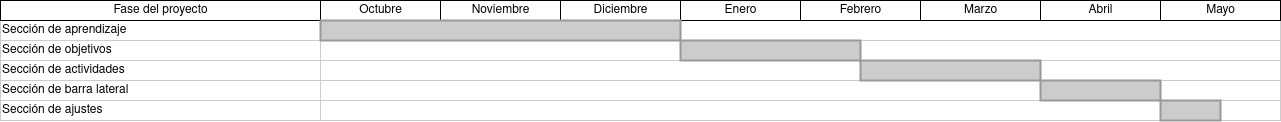
\includegraphics[scale=0.35]{img/old_Gantt.png}
	\caption{Diagrama de Gantt de las etapas del proyecto en la planificación inicial}
\end{figure}

\subsubsection{Problemas}

La planificación inicial descrita contaba con numerosos fallos, principalmente debidos a la laxitud de su definición y plazos, sumada a la incertidumbre del aprendizaje autónomo de las distintas tecnologías utilizadas. Esto, sumado a a diversos factores ajenos al proyecto, propició la necesidad de replantear el estado del mismo, y se decidió reiniciar la fase de desarrollo con una nueva planificación, ajustada esta vez a una fecha de entrega posterior, y con un nivel de detalle mucho mayor.

\subsection{Planificación final}

A mediados de abril se realizó un análisis del estado del proyecto, concluyendo en la necesidad de reiniciar su desarrollo casi por completo. Se decidió conservar la elección de tecnologías utilizadas, ya que se había dedicado una gran cantidad de tiempo a su aprendizaje. De esta forma, se ha podido obviar esta fase en la planificación final del proyecto, puesto que ya se contaba con los conocimientos necesarios para su desarrollo.

El mayor inconveniente de esta nueva planificación es el retraso en la fecha de finalización, estimada ahora el 31 de agosto de 2021. En una situación real, un retraso de varios meses como este podría causar graves consecuencias tanto al proyecto como a la reputación del desarrollador.

\subsubsection*{Distribución de etapas del proyecto en el tiempo}

Con tal de evitar los posibles imprevistos ---algo que, como ya se ha podido observar, ha afectado con severidad al proyecto anteriormente---, la nueva planificación se ha realizado de forma exhaustiva, presentando un mayor número de iteraciones, ajustadas de antemano con un listado de funcionalidades concretas a implementar.

Las etapas del proyecto quedan distribuidas de la siguiente manera:

\begin{enumerate}
	\item Investigación previa: elección de tecnologías a utilizar, revisión del estado actual del proyecto y estimación del coste de los cambios necesarios.
	
	\textbf{Plazo:} del 1 al 31 de mayo. 
	
	\item Configuración inicial del proyecto: preparación de las tecnologías elegidas y todo lo necesario para comenzar a implementar la aplicación.
	
	\textbf{Plazo:} del 22 de mayo al 7 de junio.
	
	\item Iteraciones de desarrollo o \textit{sprints}: 
	\begin{enumerate}
		\item Sprint 1: del 8 al 22 de junio.
		
		\item Sprint 2: del 23 de junio al  7 de julio.
		
		\item Sprint 3: del 8 al 21 de julio.
		
		\item Sprint 4: del 22 de julio al 5 de agosto.
		
		\item Sprint 5: del 6 al 20 de agosto.
		
		\item Sprint 6: del 21 al 31 de agosto.
	\end{enumerate}
\end{enumerate}

La distribución de las etapas en el tiempo se puede consultar en el siguiente diagrama de Gantt:

\medskip

\begin{figure}[h]
	\centering
	\includegraphics[scale=0.35]{img/gantt\ sprints.png}
	\caption{Diagrama de Gantt de las etapas del proyecto en la planificación final}
\end{figure}


\subsubsection*{Distribución de las tareas a realizar en las etapas propuestas}

A la hora de distribuir las tareas en las distintas iteraciones, se realizó una estimación de la complejidad y relevancia de cada una de las épicas del proyecto, y se planteó su implementación de forma mayormente secuencial. No obstante, la dependencia entre algunas funcionalidades obligó a adelantar el desarrollo de historias de usuario pertenecientes a épicas menos prioritarias. La última iteración se ha dedicado a realizar ajustes menores, por lo que presenta tareas de todas las épicas.

La distribución aproximada de las épicas en las iteraciones de desarrollo se puede ver en este diagrama de Gantt:

\medskip

\begin{figure}[h]
	\centering
	\includegraphics[scale=0.35]{img/gantt\ epicas.png}
	\caption{Diagrama de Gantt de las épicas del proyecto}
\end{figure}


\subsubsection*{Distribución final de las historias de usuario en las iteraciones de desarrollo}

\textbf{Sprint 1}
\begin{itemize}[leftmargin=16mm]
	\item [\textbf{TFG-9}] Como usuario, quiero crear un objetivo para poder seguirlo.
	
	\item [\textbf{TFG-10}] Como usuario, quiero poder editar un objetivo.
	
	\item [\textbf{TFG-11}] Como usuario, quiero poder actualizar el progreso de un objetivo para registrar mis hábitos.
	
	\item [\textbf{TFG-12}] Como usuario, quiero poder eliminar un objetivo de forma permanente.
	
	\item [\textbf{TFG-15}] Como usuario, quiero poder agrupar mis objetivos en categorías, para poder ordenarlos y observarlos por separado.
	
	\item [\textbf{TFG-17}] Como usuario, quiero poder ver una lista de mis objetivos actuales para tenerlos en cuenta.
	
	\item [\textbf{TFG-18}] Como usuario, quiero que el progreso de mis objetivos se reinicie una vez pasado el plazo, para poder seguirlos correctamente.

	
	\item [\textbf{TFG-19}] Como usuario, quiero poder pausar objetivos indefinidamente sin eliminarlos, para poder retomarlos en un futuro sin eliminar mis datos.
	
	\item [\textbf{TFG-67}] Como usuario, quiero ver el progreso de un objetivo para seguir mi esfuerzo.
\end{itemize}

\textbf{Sprint 2}
\begin{itemize}[leftmargin=16mm]
	\item [\textbf{TFG-14}] Como usuario, quiero poder ver una racha de cumplimiento de cada objetivo, para mantener mi motivación.

	\item [\textbf{TFG-20}] Como usuario, quiero poder ver un historial de registro de mis objetivos para poder analizarlos y ver mi progreso.
	
	\item [\textbf{TFG-21}] Como usuario, quiero ver indicadores visuales de que un objetivo se ha actualizado correctamente, o si ha habido un error, para poder actuar en consecuencia.
	
	\item [\textbf{TFG-22}] Como usuario, quiero poder ver un resumen global de mis objetivos para ver mi progreso general.
	
	\item [\textbf{TFG-24}] Como usuario, quiero poder crear una actividad para tenerla en cuenta al organizarme.
	
	\item [\textbf{TFG-25}] Como usuario, quiero poder editar una actividad para actualizar sus condiciones.
	
	\item [\textbf{TFG-26}] Como usuario, quiero poder eliminar una actividad en caso de que ya no sea de mi interés.
	
	\item [\textbf{TFG-84}] Como usuario, quiero ver la mayor racha que he alcanzado en cada objetivo para poder tener presentes mis logros.
\end{itemize}

\textbf{Sprint 3}
\begin{itemize}[leftmargin=16mm]
	\item [\textbf{TFG-16}] Como usuario, quiero poder ver un resumen de cada categoría de objetivos, para saber mi progreso con la misma.
	
	\item [\textbf{TFG-23}] Como usuario, quiero poder acceder a una vista semanal de mis actividades para poder visualizar mi tiempo.
	
	\item [\textbf{TFG-43}] Como usuario, quiero poder crear una categoría para organizar mis actividades y objetivos.
	
	\item [\textbf{TFG-44}] Como usuario, quiero poder editar una categoría si es necesario.
	
	\item [\textbf{TFG-45}] Como usuario, quiero poder asignar objetivos a una categoría, para poder ver mi progreso de forma ordenada.
	
	\item [\textbf{TFG-46}] Como usuario, quiero poder asignar actividades a una categoría, para poder ver mi semana de forma clara.
	
	\item [\textbf{TFG-87}] Como usuario, quiero poder añadir los momentos en los que practico una actividad para poder organizarme.
	
	
	\item [\textbf{TFG-88}] Como usuario, quiero poder editar los momentos en los que practico una actividad para poder ajustarlos a mi situación.
	
	\item [\textbf{TFG-89}] Como usuario, quiero poder eliminar los momentos en los que practico una actividad para poder ajustarlos a mi situación.
\end{itemize}

\textbf{Sprint 4}
\begin{itemize}[leftmargin=16mm]
	\item [\textbf{TFG-29}] Como usuario, quiero ver la fecha y hora actual para poder tenerla presente .

	\item [\textbf{TFG-30}] Como usuario, quiero ver algunos objetivos pendientes que podría completar hoy, como sugerencia por si no se me ocurre qué hacer ahora.
	
	\item [\textbf{TFG-31}] Como usuario, quiero ver un menú con las categorías que he creado, para poder acceder a la vista de categoría de cada una.
	
	\item [\textbf{TFG-32}] Como usuario, quiero disponer de un menú de navegación por las diferentes vistas de la aplicación para acceder a ellas cómodamente.
	
	\item [\textbf{TFG-33}] Como usuario, quiero poder acceder a la configuración general de la aplicación desde cualquier parte de la misma, para poder ajustar mi experiencia de forma cómoda.
	
	\item [\textbf{TFG-34}] Como usuario, quiero poder ajustar qué día y hora se reinician mis objetivos para establecer mis rutinas.
\end{itemize}

\textbf{Sprint 5}
\begin{itemize}[leftmargin=16mm]
	\item [\textbf{TFG-38}] Como usuario, quiero poder fijar una vista por defecto para que al abrir la aplicación se muestre.
	
	\item [\textbf{TFG-40}] Como usuario con problemas visuales, quiero que la aplicación sea navegable con lectores de pantalla para poder usarla cómodamente .
	
	\item [\textbf{TFG-91}] Como usuario, quiero que la vista de actividades empiece en el día de la semana configurado como inicio de semana.
\end{itemize}

\textbf{Sprint 6}
\begin{itemize}[leftmargin=16mm]
	\item [\textbf{TFG-13}] Como usuario, quiero poder definir objetivos con varios tipos de progreso, para poder flexibilizar mis objetivos .
	
	\item [\textbf{TFG-28}] Como usuario, quiero ver las actividades asociadas a una categoría en la vista de esa categoría para poder ver fácilmente cuáles son.
	
	\item [\textbf{TFG-35}] Como usuario, quiero poder establecer mi zona horaria para que el reloj y el progreso funcionen adecuadamente.
	
	\item [\textbf{TFG-37}] Como usuario, quiero poder seleccionar el tema de la aplicación para acomodarla a mis gustos y necesidades.
	
	\item [\textbf{TFG-81}] Como usuario, quiero poder ocultar el panel lateral para poder ver con mayor tamaño el resto de la aplicación.
\end{itemize}


\section{Presupuesto}

Se asume que el encargo ha sido realizado a una empresa especializada, que dispone de su propio material y 
hace frente a los costes energéticos y logísticos necesarios. Por tanto, el presupuesto aproximado que se ofrece cubre únicamente los costes
de desarrollo basados en horas de trabajo. Tampoco se tienen en cuenta impuestos aplicados.

\subsection*{Recursos humanos}

\begin{table}[h!]
	\begin{center}
		\begin{tabular}{|l|l|l|l|}
			\hline
			\rowcolor[HTML]{EFEFEF} 
			\textbf{Servicio}                   & \textbf{Tarifa (€/mes)} & \textbf{Duración (meses)} & \textbf{Total}              \\ \hline
			Salario de ingeniero informático junior a jornada completa & 1500       & 4          & \multicolumn{1}{r|}{6.000€} \\ \hline
		\end{tabular}
	\end{center}
\end{table}

Se ofrece además un presupuesto aproximado del coste de mantenimiento de la aplicación por parte del equipo de desarrollo.

\begin{table}[h!]
	\begin{center}
		\begin{tabular}{|l|l|l|l|}
			\hline
			\rowcolor[HTML]{EFEFEF} 
			\textbf{Servicio}                   & \textbf{Tarifa (€/hora)} \\ \hline
			Salario de ingeniero informático en tareas de mantenimiento & 16   \\ \hline
		\end{tabular}
	\end{center}
\end{table}
 Author Ken Schwaber, a leader in the agile process movement and a co-creator of Scrum, brings his vast expertise to helping you guide the product and software development process more effectively and efficiently. Help eliminate the ambiguity into which so many software projects are borne, where vision and planning documents are essentially thrown over the wall to developers. This high-level reference describes how to use Scrum to manage complex technology projects in detail, combining expert insights with examples and case studies based on Scrum. Emphasizing practice over theory, this book explores every aspect of using Scrum, focusing on driving projects for maximum return on investment.


\subsection*{Servicios opcionales de despliegue y mantenimiento}

Se ofrece además un presupuesto orientativo sobre el coste de desplegar y mantener la aplicación en \textit{Amazon Web Services}, utilizando instancias de coste moderado.

\begin{table}[h!]
	\begin{center}
		\begin{tabular}{|l|r|r|}
			\hline
			\rowcolor[HTML]{EFEFEF} 
			\textbf{Servicios opcionales}                                                                                                                                                           & \multicolumn{1}{l|}{\cellcolor[HTML]{EFEFEF}\textbf{Tarifa (€/hora)}} & \multicolumn{1}{l|}{\cellcolor[HTML]{EFEFEF}\textbf{Coste/año}} \\ \hline
			\begin{tabular}[c]{@{}l@{}}Despliegue de la base de datos en Amazon Aurora con una instancia \\ de tipo db.t2.medium, modelo Reserved, arrendamiento de un año, No Upfront\end{tabular} & 0,055                                                                 & 481,80€                                                         \\ \hline
			Despliegue de la aplicación en un servidor virtual Amazon EC2 de tipo r4.xlarge                                                                                                         & 0,053                                                                 & 464,28€                                                         \\ \hline
		\end{tabular}
	\end{center}
\end{table}

\subsection*{Total}

\begin{table}[h!]
	\begin{center}
		\begin{tabular}{|
				>{\columncolor[HTML]{EFEFEF}}l |l|}
			\hline
			\textbf{Total}                                          & 6.000€    \\ \hline
			\textbf{Servicios opcionales durante un año} & 946,08€ \\ \hline
		\end{tabular}
	\end{center}
\end{table}


% Capítulo: diseño y resolución del trabajo
\chapter{Desarrollo del proyecto}

\section{Consideraciones previas}

\subsection{Arquitectura de la aplicación y tecnologías utilizadas}

Se plantea una arquitectura cliente-servidor, sobre la que se implementa el patrón Modelo-Vista-Controlador \cite{Uyun2010IMPLEMENTATIONOM}.
Pese a que la implementación realizada es sencilla, este modelo permite escalar el proyecto de acuerdo a sus posibles necesidades con facilidad.

\begin{figure}[h]
	\centering
	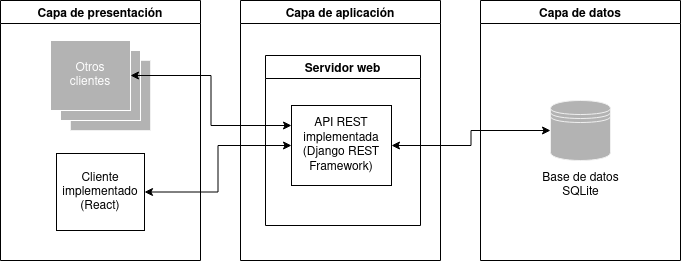
\includegraphics[scale=0.6]{img/arquitectura.png}
	\caption{Diagrama de arquitectura del proyecto}
\end{figure}

\subsubsection*{Capa de datos}

El modelo propuesto se ha implementado sobre una base de datos relacional SQLite \cite{noauthor_sqlite3_nodate}, debido a su fácil integración
con el resto de tecnologías utilizadas ---principalmente Python y Django, ya que la ofrecen de serie---;
su sencillez, dado que la base de datos se almacena en un único archivo binario; y la relativa simplicidad del modelo de datos elaborado.

En caso de ser necesario sustituir el sistema gestor de bases de datos en un futuro debido al crecimiento en complejidad de la aplicación,
es sencillo exportar SQLite a otros motores como MySQL o PostgreSQL. 
Pese a que conectar estos servicios con la aplicación resultaría sencillo ---en parte gracias a la abstracción
que realiza la capa de aplicación sobre los datos---, utilizar estas tecnologías requeriría una configuración más avanzada.

\medskip

\textbf{Alternativas exploradas}

Se eligió Django de forma rotunda en una fase bien temprana del proyecto, dado el interés en aprender a utilizarlo. En torno a la 
mitad de la fase de desarrollo, se planteó sustituir Django por Flask \cite{noauthor_flask_nodate} junto con otras tecnologías para servir 
la API, pero la idea fue descartada.

\subsubsection*{Capa de aplicación}

Se ha optado por utilizar el popular \textit{framework} de desarrollo de aplicaciones web Django para la capa de aplicación.

Su versatilidad y facilidad de uso, así como su excelente documentación y numerosa cantidad de \textit{plugins} 
desarrollados por parte de la comunidad, fueron algunos de los criterios tenidos en cuenta para su uso, además de su completa
abstracción sobre la capa de datos a la hora de gestionar el modelo.

Concretamente, la aplicación se ha construido utilizando el \textit{plugin} Django Rest Framework, que permite utilizar Django para servir
una API REST de forma sencilla, ofreciendo múltiples herramientas para trabajar con los modelos de la herramienta de forma consistente.

Se ha escogido la arquitectura REST para construir la API de la aplicación debido a su extensa acogida y soporte, así como la posibilidad
de ofrecer una documentación completa de forma estandarizada utilizando la especificación OpenAPI 3.0 \cite{miller_openapi_2021}.

\medskip

\textbf{Alternativas exploradas}

Se planteó utilizar en su lugar GraphQL \cite{noauthor_graphql_2018}, pero dada la simplicidad del modelo de datos utilizado, se descartó esta opción,
ya que no se vieron suficientes ventajas en su uso frente a REST.


\subsubsection*{Capa de presentación}

Para la capa de presentación se ha optado por desarrollar una aplicación de página única ---\textbf{SPA} por sus siglas en inglés---. Las SPA son aplicaciones
web que, por medio de AJAX u otras tecnologías similares \cite{van_kesteren_xmlhttprequest_2016}, funcionan actualizando un único documento de forma dinámica, ofreciendo una experiencia similar a una aplicación de escritorio. 

Se ha elegido utilizar React como tecnología principal para la elaboración del cliente propuesto. React es una biblioteca de código abierto orientada al desarrollo de
SPAs, creada y mantenida por Facebook. Goza de una gran popularidad, un sólido ecosistema de componentes y \textit{plugins}, y es ampliamente utilizada
en multitud de proyectos. Además, ha sido elegido el \textit{framework} de desarrollo web más popular, así como uno de los más requeridos en empresas, en la encuesta para desarrolladores de Stack Overflow de 2021 \cite{noauthor_stack_2021}.

\medskip

\textbf{Alternativas exploradas}

Junto con React, Angular y Vue.js son dos de los \textit{frameworks} de desarrollo de SPAs más populares. A la hora de escoger una de estas herramientas,
se estudió su modelo de trabajo, su popularidad \cite{potter_angular}, su curva de aprendizaje y, sobre todo, la magnitud del proyecto.

Angular, al tratarse de un \textit{framework} completo, ofrece muchas más herramientas que React, integrando muchos módulos y tecnologías útiles
de primera mano. No obstante, la sencillez de React juega a su favor, ya que adaptarse a la forma de trabajar en Angular es un proceso mucho más complejo,
y es necesario conocer los patrones de desarrollo específicos de la plataforma, como la inyección de dependencias o los servicios.

Vue.js también fue considerado, pero se descartó debido a su menor ecosistema de componentes, bibliotecas y documentación frente a las otras alternativas.


\subsection{Planteamiento de la metodología de desarrollo}

La elección de definir una metodología con principios ágiles fue clara desde el principio; no obstante, extraer elementos de las distintas opciones más populares no resultó tan sencillo, puesto que este tipo de metodologías están muy orientadas a trabajar en equipos ---generalmente pequeños, pero equipos al fin y al cabo---, con muchos elementos de comunicación, retrospectiva y revisión por parte del resto de miembros que en este caso no eran posibles.

Por ello, se hizo una selección de elementos generales, como el tablero Kanban, el desarrollo iterativo y las historias de usuario, pero dejando de lado el aspecto <<social>> de metodologías como \textit{SCRUM} o \textit{eXtreme Programming}. Dado que se trata de un encargo simulado, tampoco se ha podido contar con la perspectiva de un cliente real a lo largo del desarrollo, pero se han intentado imitar las distintas peculiaridades que pueden surgir de un encargo realizado por alguien que desconoce el proceso de desarrollo de software, tanto a través de las historias de usuario como de algunos cambios durante la implementación de la aplicación.

\newpage

\section{Iteraciones del desarrollo}

Siguiendo la planificación final propuesta, se han realizado un total de ocho iteraciones, sirviendo las dos primeras para plantear y configurar el marco de trabajo y el entorno de desarrollo, y las seis restantes dedicadas a la implementación del mismo.


\subsection{Primera y segunda iteración: investigación sobre tecnologías a utilizar y configuración inicial}

\textbf{Inicio:} 1 de mayo

\textbf{Fin:} 7 de junio

\subsubsection{Análisis}

Como se menciona en la sección de planificación, el proyecto se planteó de nuevo, aprendiendo de los errores cometidos en la primera propuesta elaborada, e intentando distinguir qué elementos mantener en la definitiva.

Se decidió elaborar una lista de historias de usuario nueva, simulando una reunión extensa con el cliente, y aclarando los requisitos de la aplicación de forma detallada, utilizando la flexibilidad de las historias de usuario. Se decidió trabajar con la herramienta \textit{Jira Software}, ya que ofrece un excelente medio de comunicación entre el equipo de desarrollo y el cliente, al mismo tiempo que una gestión del proceso de desarrollo muy completa, e integra varios de los elementos de las metodologías ágiles elegidos para el proyecto.

Después de definir la lista de historias de usuario o \textit{product backlog}, se procedió a realizar la planificación temporal. Se acordó una fecha límite para la implementación del producto mínimo viable: el 31 de agosto. Además, se decidió trabajar con iteraciones de dos semanas, con la salvedad de las dos primeras dados sus requisitos especiales, y se repartieron las distintas historias de usuario entre ellas de forma orientativa, ordenadas por categoría y prioridad.

La planificación quedó reflejada en dos diagramas de Gantt, organzizados tanto de forma temporal como por los objetivos del proyecto.


\subsubsection{Diseño}

Durante esta iteración se definió la arquitectura de la aplicación de forma concreta. Se decidió mantener la estructura utilizada anteriormente, es decir, utilizar SQLite como sistema gestor de bases de datos, Django REST Framework como aplicación del servidor, y un cliente web desarrollado con React. 

No obstante, se realizaron importantes cambios en el enfoque del proyecto. En la capa de aplicación, se decidió utilizar la especificación OpenAPI, concretamente la versión 2.0, para documentar la API expuesta. Aprovechando esto, se decidió integrar la herramienta \textit{Swagger UI} para ofrecer una forma sencilla de visualizar la documentación de la misma, así como realizar peticiones de forma cómoda durante el desarrollo.

En cuanto a los cambios del cliente, se apostó por utilizar una biblioteca de componentes prediseñados, ya que, además de agilizar el proceso de desarrollo, contienen multitud de utilidades que facilitan el diseño de la experiencia de usuario. Se contemplaron diferentes opciones, como \textit{Carbon Design System} \cite{noauthor_carbon_nodate}, desarrollado por IBM, o Material UI \cite{noauthor_material-ui:_nodate}, una implementación del sistema de diseño \textit{Material Design} \cite{noauthor_material_nodate} de Google. 

Debido a los problemas de rendimiento de Carbon Design System y su menor variedad de componentes, finalmente se optó por Material UI. Se realizaron varios bocetos y prototipos, tanto estáticos como interactivos ---estos últimos utilizando la herramienta gratuita \textit{Adobe Xd}, para definir el diseño de la aplicación y la experiencia de usuario, garantizando que las funcionalidades fuesen posibles de mostrar e implementar, y resultasen útiles al usuario final.

A continuación se muestran imágenes de los prototipos y bocetos elaborados.

\begin{figure}[hbt!]
	\centering
	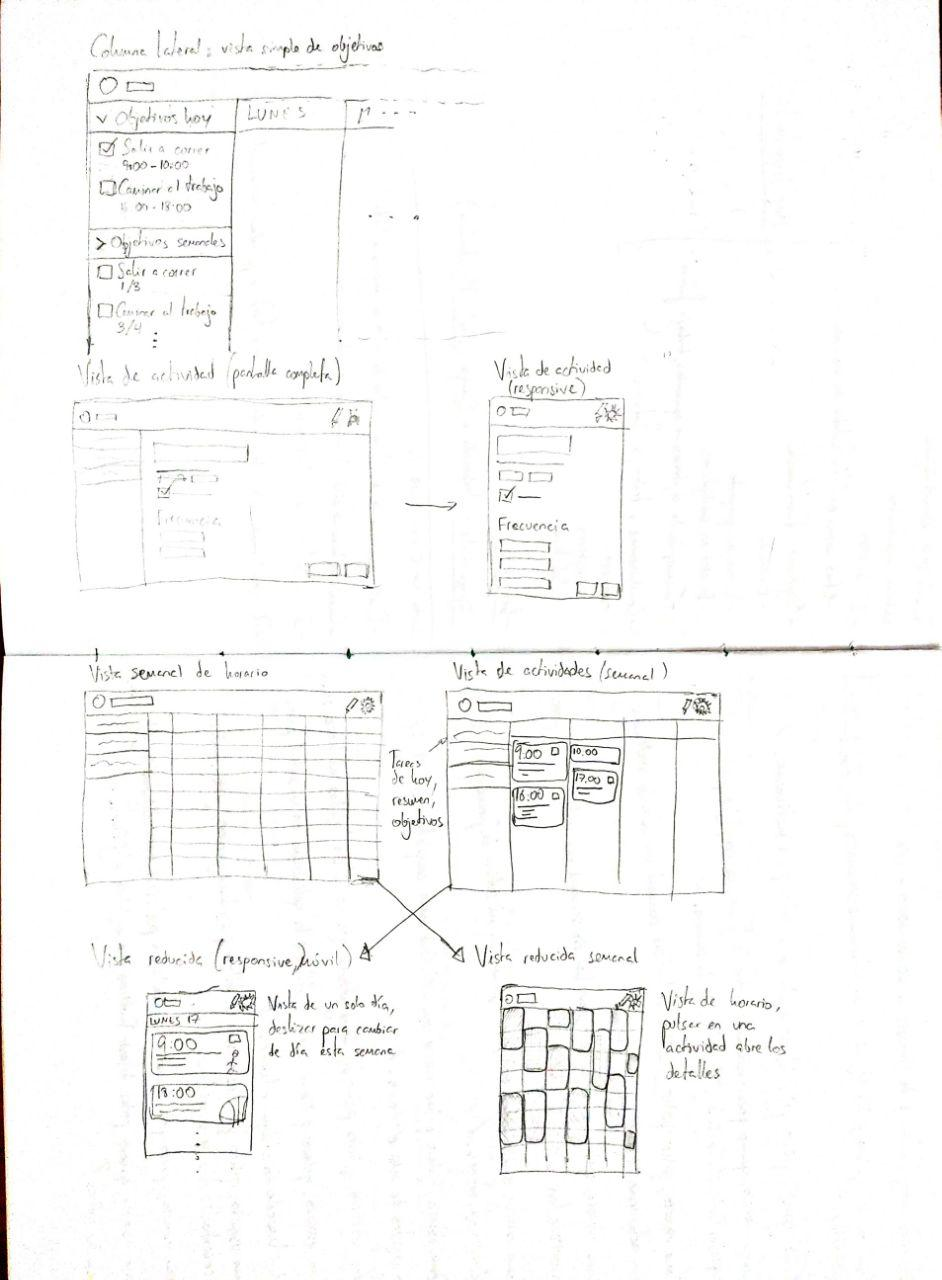
\includegraphics[scale=0.6]{img/sprint1-boceto-papel.jpg}
	\caption{Bocetos iniciales a papel}
\end{figure}

\begin{figure}[hbt!]
	\centering
	%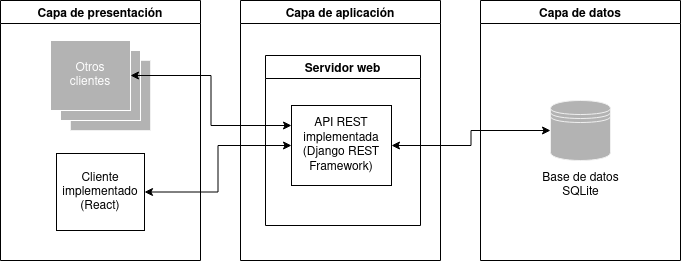
\includegraphics[scale=0.6]{img/arquitectura.png}
	\caption{Capturas de pantalla del primer prototipo interactivo}
\end{figure}

\begin{figure}[hbt!]
	\centering
	%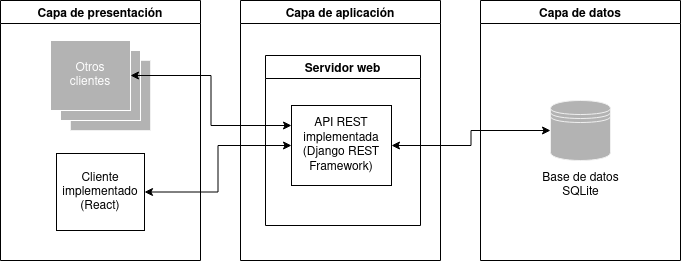
\includegraphics[scale=0.6]{img/arquitectura.png}
	\caption{Capturas de pantalla del segundo prototipo interactivo}
\end{figure}

\begin{figure}[hbt!]
	\centering
	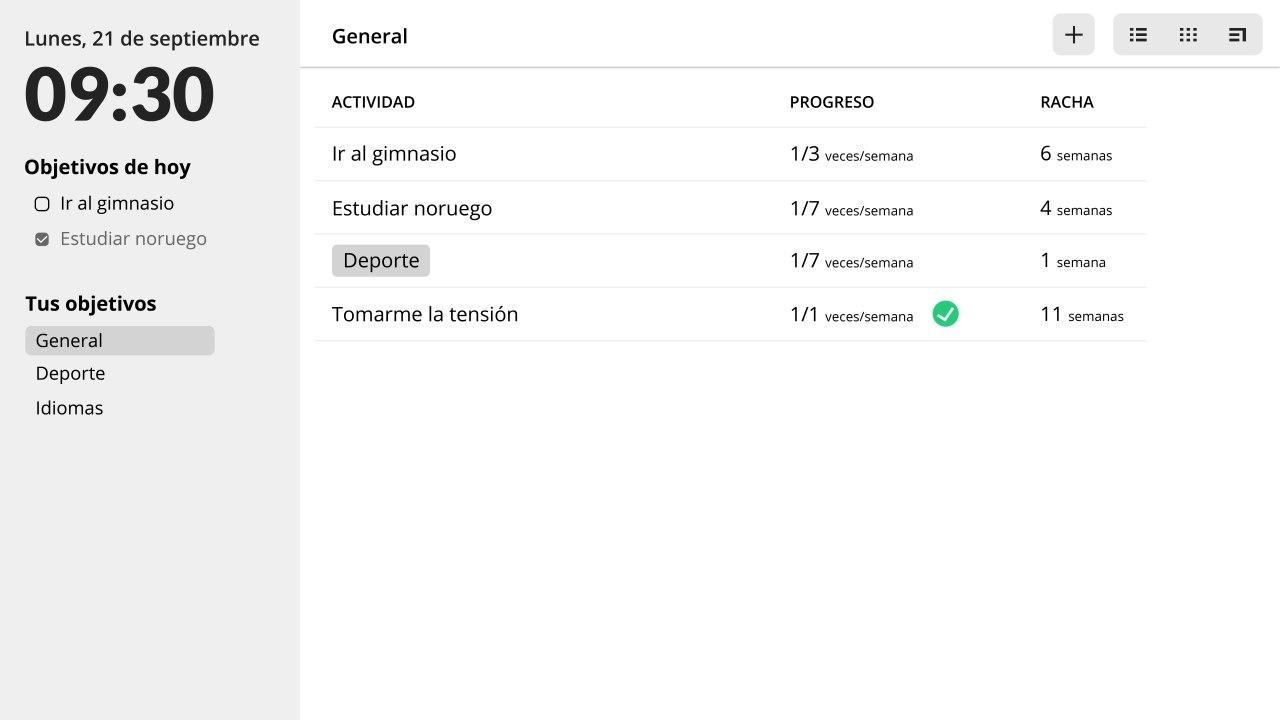
\includegraphics[scale=1.25]{img/sprint1-wireframe-objetivos.jpg}
	\caption{Boceto en alta definición de la vista de objetivos}
\end{figure}

\begin{figure}[hbt!]
	\centering
	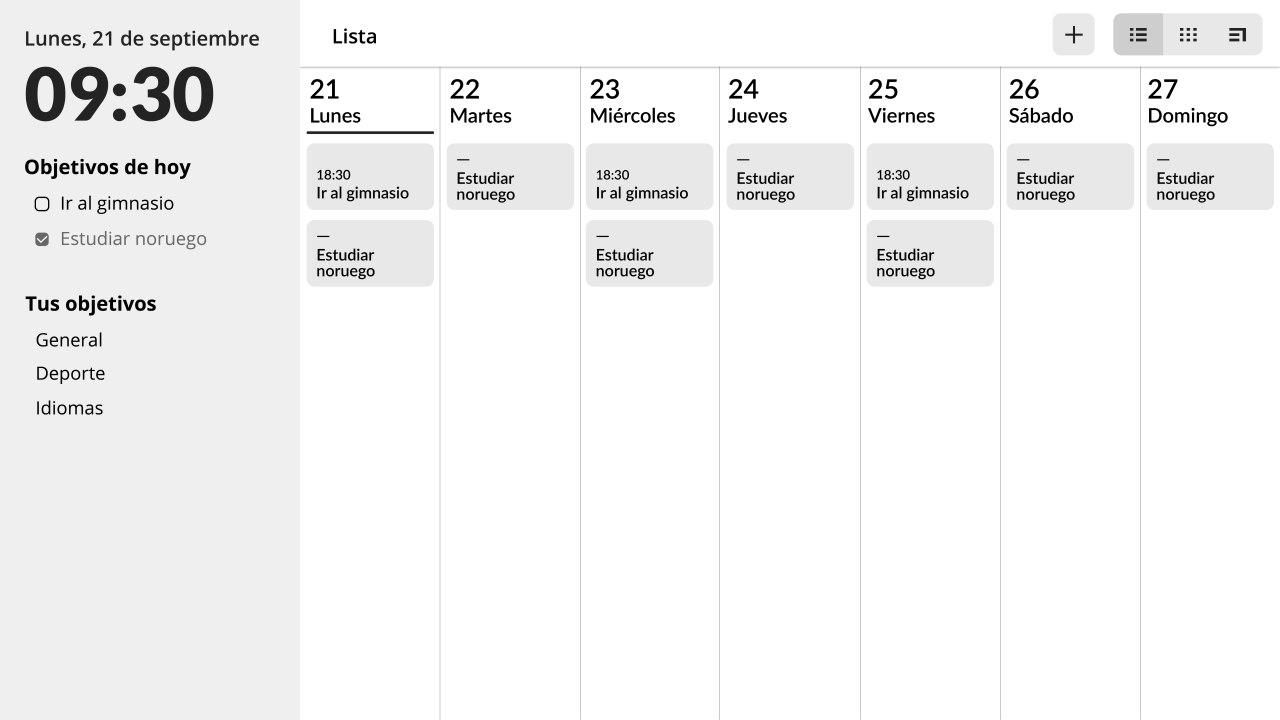
\includegraphics[scale=1.25]{img/sprint1-wireframe-lista-actividades.jpg}
	\caption{Boceto en alta definición de la vista de actividades}
\end{figure}

\begin{figure}[hbt!]
	\centering
	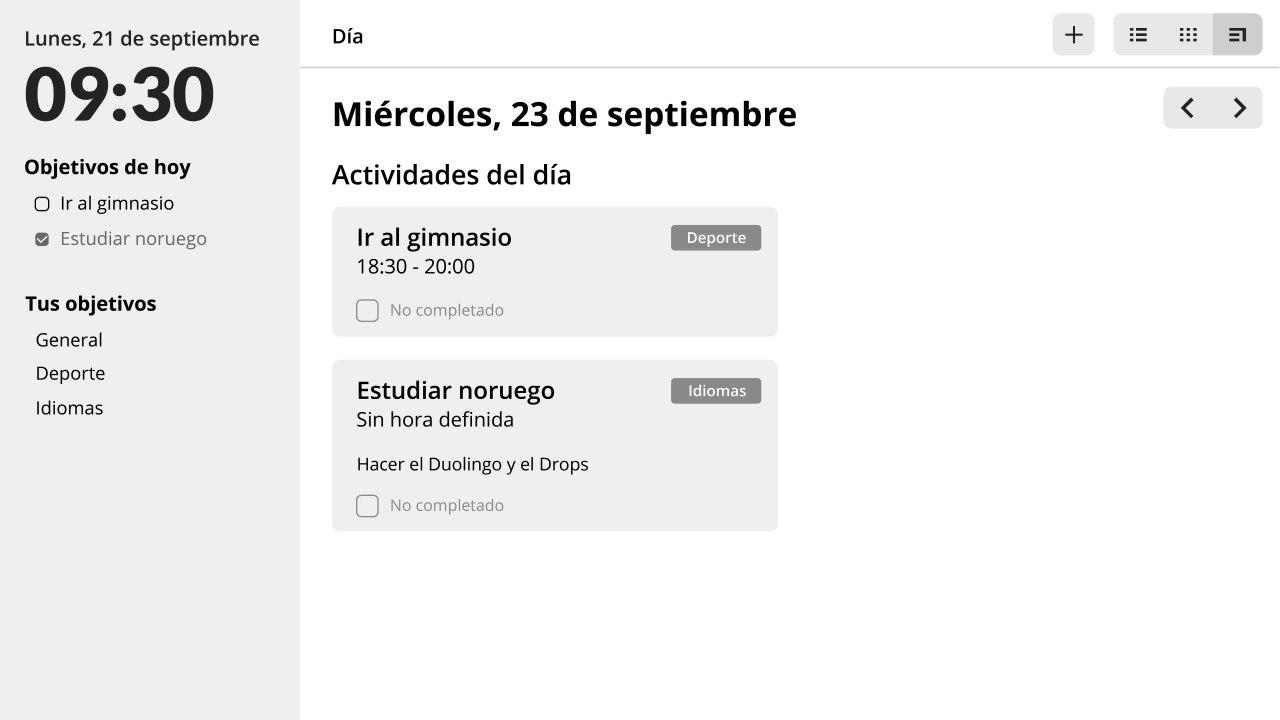
\includegraphics[scale=1.25]{img/sprint1-wireframe-actividades.jpg}
	\caption{Boceto en alta definición de la vista de día ---descartada en el diseño final---}
\end{figure}

\begin{figure}[hbt!]
	\centering
	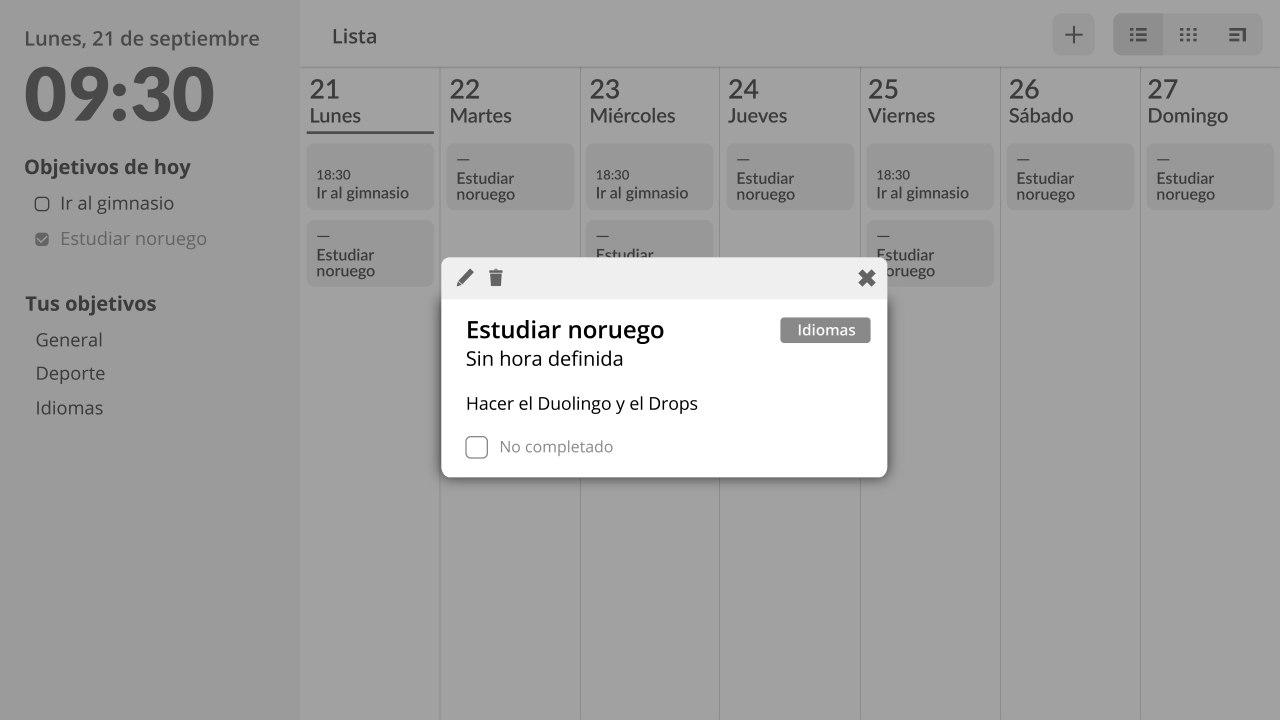
\includegraphics[scale=1.25]{img/sprint1-wireframe-popup.jpg}
	\caption{Boceto en alta definición del aspecto de las ventanas emergentes}
\end{figure}

\clearpage

\subsubsection{Implementación}

Se creó un repositorio Git alojado en la plataforma GitHub, para realizar un control de versiones del proyecto. Una vez hecho esto, se procedió a inicializar tanto el \textit{backend} como el \textit{frontend} de la aplicación con las respectivas tecnologías elegidas. Para la API, se realizó una instalación de Django tal y como describe la documentación del proyecto \cite{noauthor_how_nodate}. Para el cliente, se utilizó la herramienta \textit{create-react-app} \cite{noauthor_create_nodate}, especificando la plantilla de TypeScript.

Se instalaron las dependencias necesarias en ambos proyectos, principalmente Django REST Framework, Swagger UI ---mediante la extensión de Django \textit{drf-yasg} \cite{vijdea_drf-yasg_nodate}--- y Material UI, y se configuró el cliente para conectarse al servidor, configurando los parámetros necesarios.

Se decidió trabajar de forma local durante el desarrollo, sirviendo el cliente y el servidor en los puertos HTTP 3000 y 8000, respectivamente.

\subsubsection{Pruebas}

Una vez la configuración fue completada, se comprobó que la conexión entre el cliente y el servidor funcionaba correctamente, las dependencias se hallaban correctamente instaladas y las aplicaciones se servían en sus respectivos puertos HTTP.


\subsection{Tercera iteración: \textit{Sprint 1}}

\textbf{Inicio:} 8 de junio

\textbf{Fin:} 22 de junio


\subsubsection{Análisis}

Las historias de usuario asignadas a esta iteración fueron las siguientes:

\begin{itemize}[leftmargin=16mm]
	\item [\textbf{TFG-9}] Como usuario, quiero crear un objetivo para poder seguirlo.
	
	\item [\textbf{TFG-10}] Como usuario, quiero poder editar un objetivo.
	
	\item [\textbf{TFG-11}] Como usuario, quiero poder actualizar el progreso de un objetivo para registrar mis hábitos.
	
	\item [\textbf{TFG-12}] Como usuario, quiero poder eliminar un objetivo de forma permanente.
	
	\item [\textbf{TFG-15}] Como usuario, quiero poder agrupar mis objetivos en categorías, para poder ordenarlos y observarlos por separado.
	
	\item [\textbf{TFG-17}] Como usuario, quiero poder ver una lista de mis objetivos actuales para tenerlos en cuenta.
	
	\item [\textbf{TFG-18}] Como usuario, quiero que el progreso de mis objetivos se reinicie una vez pasado el plazo, para poder seguirlos correctamente.
	
	
	\item [\textbf{TFG-19}] Como usuario, quiero poder pausar objetivos indefinidamente sin eliminarlos, para poder retomarlos en un futuro sin eliminar mis datos.
	
	\item [\textbf{TFG-67}] Como usuario, quiero ver el progreso de un objetivo para seguir mi esfuerzo.
\end{itemize}


Se estimó su complejidad, y las tareas necesarias previas a la implementación, como la elaboración del modelo de datos para representar un \textbf{objetivo} y una \textbf{categoría}, así como la forma de actualizarlos. Para ofrecer garantías con respecto a su funcionamiento, se acordó elaborar pruebas para aquellas funcionalidades con valores calculados automáticamente, como son las historias de usuario TFG-18 y TFG-67.


\subsubsection{Diseño}

Con respecto a la experiencia de usuario, se realizó una primera aproximación a la estructura de la aplicación y la vista de objetivos, adaptando las ideas definidas en los bocetos presentados a los componentes de diseño de Material UI. 

También se comenzó a definir el modelo de datos. Debido al deseo de poder registrar el progreso de los objetivos de forma semanal, calcular su cumplimiento consecutivo y poder consultar un historial, se planteó crear dos entidades: \textbf{objetivo} y \textbf{entrada de objetivo}.
Además, dado que el objetivo puede estar asignado a una \textbf{categoría}, y es necesario fijar un día de inicio de semana, se definieron las entidades y relaciones necesarias.


\begin{figure}[h!]
	\centering
	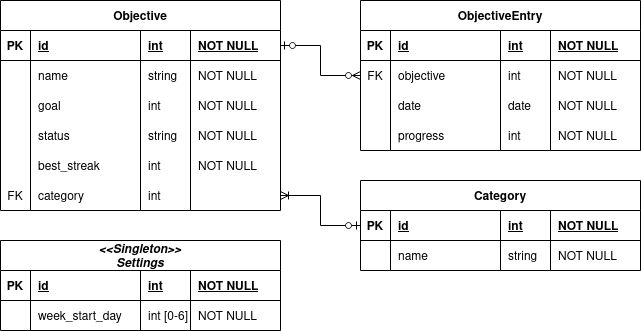
\includegraphics[scale=0.6]{img/sprint1-modelo-datos.png}
	\caption{Diagrama Entidad-Relación definido en el \textit{Sprint 1}}
\end{figure}

\subsubsection{Implementación}

Se procede a repasar los detalles de implementación de las historias de usuario asignadas.

\textbf{TFG-9}

Se creó el modelo de \textbf{objetivos} en el \textit{backend}. Django REST Framework ofrece la clase \textit{ModelViewSet}, que expone las operaciones más comunes en una API REST: crear, leer, modificar, eliminar y listar. Para ello, es necesario definir un serializador, de forma que al interactuar con la API los datos se ofrezcan en el formato deseado. Django integra funciones y clases para definir serializadores, por lo que no han sido necesarias dependencias adicionales.

Además de definir los \textit{endpoints} del modelo de objetivos, se definió el que ofrece la vista de Swagger UI.


En cuanto al \textit{frontend}, se creó el formulario de objetivos. Dado que la estructura de la aplicación no estaba plenamente definida, se priorizó el funcionamiento frente al diseño. 

Preveyendo que la aplicación contaría con multitud de ventanas emergentes y formularios similares, se optó por definir componentes genéricos, sobre los que se compondrían las diferentes variantes aprovechando las funcionalidades de React y los componentes \textit{Dialog} de Material UI.

\medskip

\textbf{TFG-10}

Debido a que Django REST Framework ofrece la funcionalidad de edición gracias a la clase \textit{ModelViewSet}, no fue necesario un gran esfuerzo en el \textit{backend}.

Sin embargo, en el \textit{frontend} se agregó al formulario definido en la historia TFG-9 la posibilidad de recibir un parámetro de entrada con un objetivo, y cambiando su funcionalidad por la de edición. Al ser la carga de datos del objetivo deseado una operación asíncrona, fue necesario asegurar que los elementos visuales aparecerían tras recibir la respuesta del servidor.

Se decidió agrupar las diferentes funciones encargadas de contactar con la API en clases, y utilizar un serializador, \textit{dcerialize} \cite{noauthor_dcerialize_nodate}, para poder trabajar de forma más flexible con los datos recibidos. 

\medskip

\textbf{TFG-11}

En esta tarea se definió el modelo de \textbf{entrada de objetivo}, de forma similar a la creación del modelo de objetivo, proporcionando las rutas creadas por \textit{ModelViewSet}. Dada su estrecha relación con el mismo, se decidió incluir dos \textit{endpoints} adicionales a modo de <<atajo>>: 

\begin{itemize}
	\item \textbf{[GET] /objectives/\{id\}/entries}, para listar las entradas asociadas a un objetivo
	\item \textbf{[POST] /objectives/\{id\}/entries}, para crear una nueva entrada asociada a un objetivo
\end{itemize}

Se implementó el modelo de entradas de objetivo en el cliente, así como la clase encargada de llamar a los distintos \textit{endpoints} de la API y el formulario de creación y edición, reutilizando los componentes previamente desarrollados.

\medskip

\textbf{TFG-12}

Debido a que esta funcionalidad viene implementada por defecto al utilizar la clase \textit{ModelViewSet} de Django REST Framework, no fue necesario hacer cambios en la API.

En el cliente, se definió un componente genérico destinado a confirmar operaciones de borrado, indicándole la operación a ejecutar al confirmar, así como distintos parámetros. Se colocó un botón provisional en la aplicación para borrar objetivos, dado que la completa implementación de esta tarea dependía de representar la lista completa. Una vez estuvo lista, se incluyó un botón en cada una de las entradas, que la elimina usando el componente de confirmación mencionado. 

\medskip

\textbf{TFG-15}

Se crearon tanto el modelo de Django como el \textit{ModelViewSet} asociados a la entidad \textbf{categoría}, añadiendo la clave externa al modelo de objetivo. Posteriormente se definieron el serializador y la documentación de OpenAPI, de forma similar a las otras dos entidades. Se creó una categoría de prueba en la base de datos para continuar el desarrollo.

En el cliente, se añadió el campo \textbf{categoría} en el modelo de objetivo y el formulario asociado. Al seleccionarlo, un desplegable muestra las distintas categorías definidas por el usuario, así como la opción \textit{Ninguna}. 

\medskip

\textbf{TFG-17}

Se decidió utilizar el componente \textit{Table} de Material UI para mostrar la lista de objetivos, encapsulándolo en otro componente dedicado a obtener la información de la API, así como controlar el renderizado condicional.

\medskip

\textbf{TFG-18}

Se añadió una propiedad nueva al modelo de objetivo, el \textbf{progreso}, calculado en función del número de entradas añadidas en la semana actual. Para ello fue necesario implementar el modelo de \textbf{configuración}, ya que contiene el día de inicio de semana, y varias funciones dedicadas a consultar la base de datos y sumar el progreso. Gracias al decorador \textit{@Property} de Django, fue sencillo añadir la propiedad calculada al modelo.

Se actualizó la documentación y el cliente para reflejar los cambios, añadiendo una columna nueva a la lista de objetivos.

\medskip

\textbf{TFG-19}

Se añadió un nuevo \textit{endpoint} a la API destinado a cambiar el estado de un objetivo, y se definió un enumerado conteniendo los distintos valores posibles. En el cliente se añadió un botón a cada entrada de la lista de objetivos dedicado a pausar y reanudar cada uno de ellos, actualizando la base de datos.

No obstante, pausar y reanudar objetivos suponía un cambio drástico en la forma de calcular el progreso, así como las rachas de cumplimiento. Se decidió posponer la implementación de esta funcionalidad de forma indefinida.

\medskip

\textbf{TFG-67}

Esta funcionalidad quedó implementada junto con la historia de usuario \textbf{TFG-18}.


\subsubsection{Pruebas}

Se elaboraron pruebas de aceptación para las tareas de cálculo del progreso semanal, TFG-18 y TFG-67, utilizando la herramienta \textit{unittest} de Python.

Dado que son funcionalidades dependientes de la fecha en la que se ejecutan, se optó por representar en las pruebas los casos límite, y utilizar la biblioteca \textit{FreezeGun} \cite{pulec_freezegun_nodate} para fijar las fechas utilizadas.


\subsection{Cuarta iteración: \textit{Sprint 2}}

\textbf{Inicio:} 23 de junio

\textbf{Fin:} 7 de julio

\subsubsection{Análisis}

Las historias de usuario asignadas a esta iteración fueron las siguientes:

\begin{itemize}[leftmargin=16mm]
	\item [\textbf{TFG-14}] Como usuario, quiero poder ver una racha de cumplimiento de cada objetivo, para mantener mi motivación.
	
	\item [\textbf{TFG-20}] Como usuario, quiero poder ver un historial de registro de mis objetivos para poder analizarlos y ver mi progreso.
	
	\item [\textbf{TFG-21}] Como usuario, quiero ver indicadores visuales de que un objetivo se ha actualizado correctamente, o si ha habido un error, para poder actuar en consecuencia.
	
	\item [\textbf{TFG-22}] Como usuario, quiero poder ver un resumen global de mis objetivos para ver mi progreso general.
	
	\item [\textbf{TFG-24}] Como usuario, quiero poder crear una actividad para tenerla en cuenta al organizarme.
	
	\item [\textbf{TFG-25}] Como usuario, quiero poder editar una actividad para actualizar sus condiciones.
	
	\item [\textbf{TFG-26}] Como usuario, quiero poder eliminar una actividad en caso de que ya no sea de mi interés.
	
	\item [\textbf{TFG-84}] Como usuario, quiero ver la mayor racha que he alcanzado en cada objetivo para poder tener presentes mis logros.
\end{itemize}

Al igual que en la iteración anterior, se estimó la complejidad de las tareas, y fueron implementadas según la prioridad asignada en la planificación.

Se mantuvo la intención de elaborar tests para las funcionalidades de los objetivos dependientes de la fecha, es decir, las historias de usuario TFG-14 y TFG-84.

\subsubsection{Diseño}

Se amplió el modelo de datos para representar la entidad de \textbf{actividades}, quedando el modelo de datos de la siguiente forma:

\begin{figure}[h!]
	\centering
	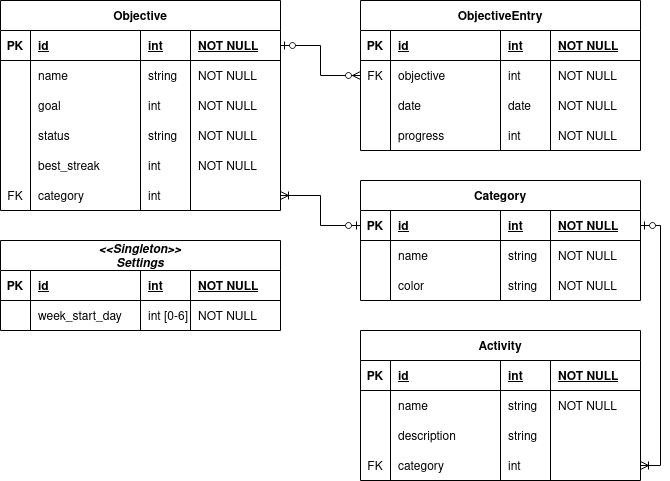
\includegraphics[scale=0.6]{img/sprint2-modelo-datos.png}
	\caption{Diagrama Entidad-Relación actualizado en el \textit{Sprint 2}}
\end{figure}


Se definió también la vista de actividades, ajustándose de nuevo a los bocetos elaborados, y se continuó utilizando Material UI sin grandes modificaciones. Además, se definieron los colores provisionales de la aplicación, utilizando la paleta de colores de Material Design \cite{noauthor_materialcolor_nodate}:

\begin{itemize}
	\item Color principal: verde 500 \medspace \tikz\draw[green500,fill=green500] (0,0) circle (.75ex);
	\item Color secundario: marrón 500 \medspace \tikz\draw[brown500,fill=brown500] (0,0) circle (.75ex);
\end{itemize}

Además, se estableció el diseño del historial de entradas de objetivos. Funcionaría a través de un calendario, cuyos días con entradas registradas aparecerían coloreados.
Al seleccionar una fecha, una ventana emergente mostaría una lista con información sobre las entradas, y un menú para poder modificarlas o eliminarlas.

\begin{figure}[h!]
	\centering
	%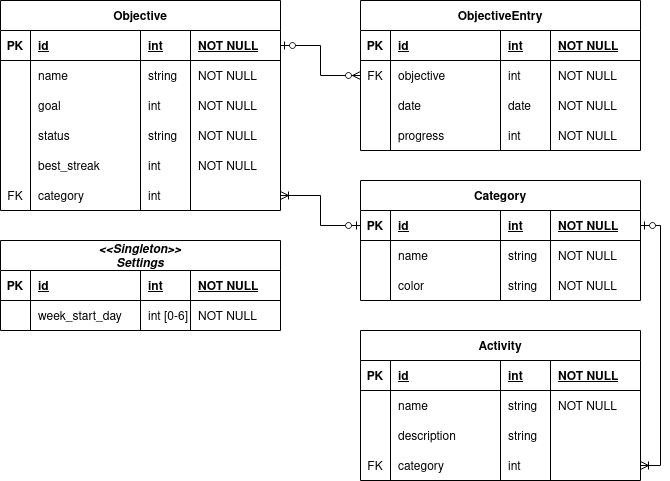
\includegraphics[scale=0.6]{img/sprint2-modelo-datos.png}
	\caption{Boceto a mano del historial de entradas de objetivo}
\end{figure}


\subsubsection{Implementación}

Se detallan a continuación las diferentes historias de usuario abordadas en esta iteración.

\textbf{TFG-14}

Se implementó esta funcionalidad haciendo uso del decorador \textit{@Property} de Django, al igual que el progreso de un objetivo. La función utilizada realiza un recorrido semana a semana, desde la actual hacia atrás, incrementando la racha de cumplimiento de un objetivo hasta encontrar una semana en la que no se haya completado.

Se plantearon opciones para guardar este valor y evitar cálculos, pero debido a la baja densidad de datos estimada para la aplicación, se determinó que supondría un esfuerzo innecesario de momento, y perjudicaría el ritmo del proyecto.

Se realizaron pequeños ajustes a la función de cálculo del progreso de un objetivo, de cara a reutilizarla en otras partes del código.

En el cliente, se añadió una columna a la lista de objetivos, así como el campo correspondiente en el modelo y el serializador, para mostrar el valor calculado.

\medskip

\textbf{TFG-20}

Para esta funcionalidad se decidió utilizar la herramienta \textit{React-Calendar} \cite{maj__react-calendar_nodate}, debido a su simplicidad, capacidad de configuración y facilidad de integración con el proyecto. 

Desde la aplicación de la API se hicieron modificaciones a las rutas del modelo de objetivo para cumplir con los requisitos de la tarea:

\begin{itemize}
	\item \textbf{(Nuevo) [GET] /objective-entries/days/} 
	
	Devuelve los días en los que hay entradas registradas.
	
	\textbf{Parámetros}
	
	\begin{itemize}
		\item \textbf{month:} entero positivo entre 1 y 12. Mes del cual se solicitan los días. Si no se especifica, se devuelven los resultados del mes actual.
	\end{itemize}

	\item \textbf{(Modif.) [GET] /objective-entries/} 
	
	Devuelve una lista con las entradas registradas.

	\textbf{Parámetros}
	
	\begin{itemize}
		\item \textbf{date:} fecha en formato ISO 8601 \cite{houston1993iso}. Se devolverán los resultados con la fecha indicada.
	\end{itemize}
\end{itemize}

\medskip

Desde el cliente, se instaló el paquete \textit{React-Calendar}, y se plantearon los siguientes componentes, encargados de implementar la funcionalidad deseada:

\begin{itemize}
	\item \textbf{ObjectiveEntryCalendar:} componente encargado de representar el calendario de entradas, mostrar los días disponibles y solicitar a la API los datos necesarios una vez seleccionado un día.
	
	\item \textbf{ObjectiveEntryHistory:} lista de entradas representadas utilizando componentes \textit{Card} de Material UI, mostrando la información de cada una de ellas. El menú contextual para editar y borrar una entrada se implementaría más adelante.
	
	\item \textbf{EntryHistoryDialog:} componente derivado de los previamente desarrollados para presentar ventanas emergentes. Muestra el historial de entradas al seleccionar una fecha en el calendario.
\end{itemize}


\medskip

\textbf{TFG-21}

En esta tarea se añadieron los indicadores de progreso \textit{CircularProgress} proporcionados por Material UI, para representar la espera de respuesta por parte del servidor. Se colocaron en todos los componentes que necesitasen actualizar datos, ya que antes, pese a actualizarse correctamente, el usuario no tenía forma de saber que la aplicación estaba esperando datos.

\medskip

\textbf{TFG-22}

En esta tarea se integró el componente de historial implementado en la historia \textbf{TFG-20} en la vista de objetivos, de forma que todo lo relacionado con objetivos se encuentra en la misma vista. 

\medskip

\textbf{TFG-24}

Para implementar esta tarea se definió en modelo de actividades en Django siguiendo el mismo proceso que los anteriores, y generando una vista con la clase \textit{ModelViewSet}, que proporciona las rutas básicas de la API. Se hizo lo mismo en la parte del cliente, definiendo el modelo, serializador y funciones de consulta. 

Dado que la vista de actividades no estaba lista, se realizó la implementación del formulario de creación/edición de actividad partiendo de los ya existentes, pero no se introdujo en la aplicación de forma definitiva. Una vez añadida la funcionalidad de añadir instancias de la actividad en la vista correspondiente, se volvería a abrir esta tarea, para completarla definitivamente.

\medskip

\textbf{TFG-25}

Esta funcionalidad se implementó junto con la creación de actividades en la historia \textbf{TFG-24}, debido a la reutilización de componentes.

\medskip

\textbf{TFG-26}

Dado que se definió un componente de confirmación para operaciones potencialmente destructivas, y la existencia previa del \textit{endpoint} de borrado para el modelo de actividad, la implementación de esta tarea consistió en añadir una función de borrado para utilizarla con el componente de confirmación. Al igual que la historia \textbf{TFG-24}, quedaría pendiente de integrar en la aplicación una vez la vista de actividades estuviese lista.

\medskip

\textbf{TFG-84}

Para la realización de esta tarea se definió una función en el servidor dedicada a incrementar el campo correspondiente del modelo de objetivo. Utilizando la funcionalidad de \textbf{señales} \cite{noauthor_signals_nodate} de Django, se estableció que la función se ejecutaría al añadir progreso en un objetivo. Si se había completado, actualizaría la mejor racha con el valor de la racha actual, siempre y cuando fuese mayor al valor almacenado.

Dado que al editar un objetivo se puede cambiar la meta del mismo, se producían inconsistencias en los datos, pudiendo aumentar de forma artificial la mejor racha alcanzada. Para evitar esto, se estableció otra señal, que calcula de nuevo la mejor racha si la meta de un objetivo es modificada.

No fue necesario realizar modificaciones en el cliente, ya que este dato se encontraba en el modelo, y se mostraba en la lista de objetivos.

\medskip

\subsubsection{Pruebas}

Al igual que con las historias anteriores relacionadas con los cálculos automáticos de los datos de objetivos, se diseñaron tests \textit{a priori} para las funcionalidades implementadas en las historias TFG-14 y TFG-84 con la utilidad \textit{unittest} de Python.


\subsection{Quinta iteración: \textit{Sprint 3}}

\textbf{Inicio:} 8 de julio

\textbf{Fin:} 21 de julio

\subsubsection{Análisis}

Las historias de usuario asignadas a esta iteración fueron las siguientes:

\begin{itemize}[leftmargin=16mm]
	\item [\textbf{TFG-16}] Como usuario, quiero poder ver un resumen de cada categoría de objetivos, para saber mi progreso con la misma.
	
	\item [\textbf{TFG-23}] Como usuario, quiero poder acceder a una vista semanal de mis actividades para poder visualizar mi tiempo.
	
	\item [\textbf{TFG-43}] Como usuario, quiero poder crear una categoría para organizar mis actividades y objetivos.
	
	\item [\textbf{TFG-44}] Como usuario, quiero poder editar una categoría si es necesario.
	
	\item [\textbf{TFG-45}] Como usuario, quiero poder asignar objetivos a una categoría, para poder ver mi progreso de forma ordenada.
	
	\item [\textbf{TFG-46}] Como usuario, quiero poder asignar actividades a una categoría, para poder ver mi semana de forma clara.
	
	\item [\textbf{TFG-87}] Como usuario, quiero poder añadir los momentos en los que practico una actividad para poder organizarme.
	
	\item [\textbf{TFG-88}] Como usuario, quiero poder editar los momentos en los que practico una actividad para poder ajustarlos a mi situación.
	
	\item [\textbf{TFG-89}] Como usuario, quiero poder eliminar los momentos en los que practico una actividad para poder ajustarlos a mi situación.
\end{itemize}

Se priorizó el desarrollo de la historia TFG-23, dado que en el sprint anterior se comenzaron a implementar dos tareas que dependían de su finalización. Se vio que el desarrollo de las operaciones de creación y edición de categorías presentarían un problema similar, puesto que aún quedaría pendiente implementar la barra lateral, donde aparecerían listadas. No obstante, se consideró que era más importante garantizar el correcto funcionamiento de los datos y su manejo, y dejar la presentación para más adelante.

Se puede observar que la historia de usuario TFG-45 es un duplicado de la ya implementada TFG-15, por lo que se decidió marcarla como completada y no tenerla en cuenta.


\subsubsection{Diseño}

Es en esta iteración cuando se define formalmente la entidad \textbf{instancia de actividad}, entendiéndose como una repetición de una actividad en un horario semanal fijo, con día, hora de inicio y hora de finalización.

Tras las modificaciones realizadas, el modelo de datos quedó definido de la siguiente forma:

\begin{figure}[h!]
	\centering
	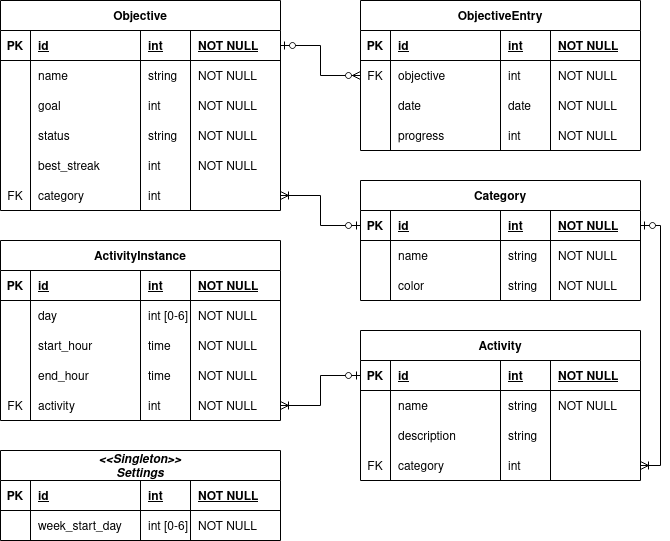
\includegraphics[scale=0.6]{img/sprint3-modelo-datos.png}
	\caption{Diagrama Entidad-Relación actualizado en el \textit{Sprint 3}}
\end{figure}


\subsubsection{Implementación}

\textbf{TFG-16}

Para la implementación de esta tarea se decidió ofrecer un filtro de la vista de objetivos actual, mostrando únicamente la información de los objetivos asociados con la categoría seleccionada. Para ello, se añadió la posibilidad de filtrar los datos desde la API, añadiendo el parámetro \textit{category} a las rutas de listado tanto de objetivos como de entradas.

Desde el cliente, se añadió una propiedad opcional a los distintos componentes que forman la vista de objetivos para recibir una categoría. Si esta propiedad se hallaba definida, era enviada como parámetro al solicitar los datos. 

Surgió la idea de utilizar el color de las categorías para sobreescribir el tema de la aplicación al filtrar la vista de objetivos, por lo que se añadió una nueva historia de usuario al \textit{backlog}, aunque de baja prioridad.

Dado que la barra lateral aún no estaba completada, las pruebas de implementación se realizaron sobre una lista provisional de categorías. Una vez estuviese terminada, se implementaría el filtrado al seleccionar un elemento de la lista.

\medskip

\textbf{TFG-23}

Para la implementación de la vista semanal se decidió utilizar un diseño muy similar al propuesto en los bocetos digitales, mostrando una lista flexible de tarjetas que contienen la información sobre las diferentes instancias, su horario y su categoría. 

Dado que la funcionalidad de listado de actividades e instancias en el servidor ya se había implementado con anterioridad, esta tarea se centró en el cliente. La vista se construyó utilizando flexbox \cite{noauthor_flexbox_nodate} y los componentes auxiliares proporcionados por Material UI.

Una vez finalizada la implementación de la vista, se colocaron en ella los botones y formularios necesarios para crear actividades e instancias, así como un menú desplegable en cada tarjeta para permitir la edición y el borrado. Las funcionalidades de listado, edición y borrado de actividades seguirían pendientes de ser integradas en la aplicación hasta que la barra lateral fuese implementada.

\medskip

\textbf{TFG-43}

Dado que el modelo de categorías llevaba creado en la base de datos desde la primera iteración debido a su relación con el modelo de objetivos, las operaciones básicas de la API con respecto a él ya se encontraban definidas. Al igual que otras tareas similares, el desarrollo se centró en reutilizar los componentes de formularios y ventanas emergentes definidos y adaptarlos al modelo de categorías. 

De nuevo, la integración de esta funcionalidad en la aplicación quedó pendiente del desarrollo de la barra lateral, ya que tanto la lista de categorías como el botón de creación de las mismas se colocaría en ella. 

\medskip

\textbf{TFG-44}

Esta funcionalidad ya había sido incluida en la historia TFG-43, debido a la reutilización de componentes previos.

\medskip

\textbf{TFG-46}

Pese a que no se había definido como tarea en la épica de actividades, al crear el modelo de datos se tuvo en cuenta la posibilidad de asignar una categoría a una actividad, por lo que esta historia de usuario ya se encontraba completada.

\medskip

\textbf{TFG-87}

Para implementar esta funcionalidad, se añadió el modelo de \textbf{instancia de actividad}. Al igual que el resto de entidades de datos, se creó un modelo de Django, junto con las respectivas rutas de la API generadas por \textit{ModelViewSet} en el servidor, y las distintas funciones y definiciones necesarias en el cliente.

Sin embargo, en lugar de crear un nuevo formulario, se decidió expandir el ya creado para las actividades, implementando una sección condicional. Se añadió un campo que permitía seleccionar entre crear una actividad o seleccionar una ya existente. Al elegir crear una nueva, aparecerían los campos del formulario de nueva actividad, seguidos de los necesarios para crear una instancia, y se crearían ambos elementos. En caso contrario, aparecerían únicamente los de la instancia.

\medskip

\textbf{TFG-88}

Debido a la peculiaridad del formulario de creación de instancias de actividades, fue necesario elaborar un componente aparte para modificarlas, a diferencia del resto de modelos de la aplicación. Dicho formulario contiene únicamente los campos relativos a la instancia, es decir, día de la semana, hora de inicio y hora de finalización. La funcionalidad del servidor permaneció intacta.

\medskip

\textbf{TFG-89}

Al igual que el resto de operaciones destructivas, se implementó esta funcionalidad instanciando el componente de confirmación, utilizando la función de borrado definida junto con el modelo.


\subsubsection{Pruebas}

Se planteó implementar tests para comprobar el funcionamiento de todos los \textit{endpoints} de la API, pero dado que la mayoría de ellos eran servidos de forma automática por Django REST Framework y el resto correspondían a funcionalidades ya cubiertas en otros tests, se decidió descartar la idea.

Se comprobó que los tests definidos eran superados correctamente.


\subsection{Sexta iteración: \textit{Sprint 4}}

\textbf{Inicio:} 22 de julio

\textbf{Fin:} 5 de agosto


\subsubsection{Análisis}

Las historias de usuario asignadas a esta iteración fueron las siguientes:

\begin{itemize}[leftmargin=16mm]
	\item [\textbf{TFG-29}] Como usuario, quiero ver la fecha y hora actual para poder tenerla presente .
	
	\item [\textbf{TFG-30}] Como usuario, quiero ver algunos objetivos pendientes que podría completar hoy, como sugerencia por si no se me ocurre qué hacer ahora.
	
	\item [\textbf{TFG-31}] Como usuario, quiero ver un menú con las categorías que he creado, para poder acceder a la vista de categoría de cada una.
	
	\item [\textbf{TFG-32}] Como usuario, quiero disponer de un menú de navegación por las diferentes vistas de la aplicación para acceder a ellas cómodamente.
	
	\item [\textbf{TFG-33}] Como usuario, quiero poder acceder a la configuración general de la aplicación desde cualquier parte de la misma, para poder ajustar mi experiencia de forma cómoda.
	
	\item [\textbf{TFG-34}] Como usuario, quiero poder ajustar qué día se reinician mis objetivos para establecer mis rutinas.
\end{itemize}

\medskip

En este sprint se implementarían las tareas relativas a la \textbf{barra lateral}, desbloqueando las historias de usuario que quedaban pendientes de completar:

\begin{itemize}[leftmargin=16mm]
	\item[\textbf{TFG-43}] Creación de categorías
	\item[\textbf{TFG-44}] Edición de categorías
	\item[\textbf{TFG-25}] Edición de actividades
	\item[\textbf{TFG-26}] Borrado de actividades
\end{itemize}

Además, se añadiría la sección de configuración de la aplicación, una funcionalidad que ya estaba implementada en la parte del servidor, pero que era imposible modificar desde el cliente hasta ahora.


\subsubsection{Diseño}

Todas las funcionalidades de esta iteración pertenecen al cliente, salvo la historia TFG-30, para la cual se planteó devolver, a través de un nuevo \textit{endpoint} de la API, una pareja de objetivos sin completar, uno de ellos cerca de su finalización y otro aún no comenzado o con menos progreso registrado.

Aparte de esto, la capa de aplicación no sufrió modificaciones en esta iteración, ya que la funcionalidad de la historia TFG-34 fue implementada en las funciones de progreso y cálculo de rachas del modelo de objetivo.

Para el aspecto visual y la experiencia de usuario del cliente, se partió de nuevo de los bocetos digitales proporcionados, aunque con ligeras modificaciones, como trasladar los botones de navegación a la barra lateral ---en lugar de hallarse en la barra de título, como figuraban en los bocetos---.


\subsubsection{Implementación}

\textbf{TFG-29}

Para implementar esta funcionalidad se añadió la \textbf{barra lateral}, aunque vacía, y se colocó un reloj digital y la fecha actual en la parte superior.

Se realizaron los ajustes de estilo necesarios en el resto de la aplicación.

\medskip

\textbf{TFG-30}

Se implementó un nuevo\textit{endpoint} en la API, \textbf{[GET] /objectives/suggestions}, que devuelve una lista con dos objetivos: el de mayor y menor progreso. Se implementó la función necesaria en el \textit{ModelViewSet} de objetivo, con su correspondiente documentación. 

En el cliente se creó la función encargada de contactar con la API y deserializar los datos, además del componente de lista de sugerencias, que iría embebido en la barra lateral, mostrando un botón para añadir progreso en cada uno de los elementos. Al pulsar el botón, se mostraría el formulario de creación de entrada de objetivo.

\medskip

\textbf{TFG-31}

Se elaboró un componente en el cliente para mostrar la lista de las categorías disponibles, integrándolo con las capacidades de listado ya implementadas en el servidor. Se colocó en la barra lateral, y se realizaron los ajustes de CSS necesarios para que, en caso de desbordamiento, el desplazamiento se produjese únicamente en la lista, y no en toda la barra lateral. Esto se consiguió utilizando flexbox, junto con otras propiedades CSS.

\medskip


\textbf{TFG-32}

Se añadió un grupo de botones exclusivos a la barra lateral, bajo el reloj digital, encargados de controlar la vista mostrada. Para conseguir esto, se investigó sobre la API de contexto de React \cite{noauthor_context_nodate}, y se implementó un contexto global para la aplicación, responsable de controlar los parámetros globales de la misma, y almacenar datos compartidos por numerosos componentes.

\medskip


\textbf{TFG-33}

Se añadió un botón estilizado en la parte inferior de la barra lateral, el cual muestra un formulario con las diferentes opciones de configuración. Durante la implementación de esta tarea, únicamente se mostraba el día de inicio de semana, como un desplegable.

Debido al desajuste entre los formatos de fecha y hora de TypeScript y Python ---la semana en TypeScript comienza en domingo, mientras que en Python lo hace en lunes---, fue necesario solucionarlo de forma manual.

\medskip

\textbf{TFG-34}

Esta tarea ya se encontraba implementada en el modelo de objetivo, y al ser necesaria para implementar la historia TFG-33, lo único necesario para finalizarla fue incluir el campo correspondiente en el formulario de configuración.

\medskip


\subsubsection{Pruebas}

Las pruebas relativas al reinicio de progreso en diferentes fechas ya se encontraban implementadas, por lo que no fue necesario repetirlas.

Todos los tests se mantenían superados al finalizar la implementación de esta iteración, y se simuló una reunión con el cliente para confirmar el correcto desarrollo del proyecto.



\subsection{Séptima iteración: \textit{Sprint 5}}

\textbf{Inicio:} 6 de agosto

\textbf{Fin:} 20 de agosto


\subsubsection{Análisis}

Las historias de usuario asignadas a esta iteración fueron las siguientes:

\begin{itemize}[leftmargin=16mm]
	\item [\textbf{TFG-38}] Como usuario, quiero poder fijar una vista por defecto para que al abrir la aplicación se muestre.
	
	\item [\textbf{TFG-40}] Como usuario con problemas visuales, quiero que la aplicación sea navegable con lectores de pantalla para poder usarla cómodamente.
	
	\item [\textbf{TFG-91}] Como usuario, quiero que la vista de actividades empiece en el día de la semana configurado como inicio de semana.
\end{itemize}

Debido a que la fecha de finalización se aproximaba, se acordó destinar un menor número de historias de usuario a las últimas iteraciones, y dedicar el resto de esfuerzos a solucionar posibles errores y mejorar la presentación de la aplicación.

 
\subsubsection*{Diseño}

Se analizaron los problemas de contraste de la aplicación con las herramientas de desarrollo web integradas en el navegador Firefox \cite{noauthor_firefox_nodate} para corregirlos en la implementación de la historia TFG-40, y se decidió modificar el modelo de configuración en la base de datos para guardar la vista por defecto de la aplicación.

\begin{figure}[hbt!]
	\centering
	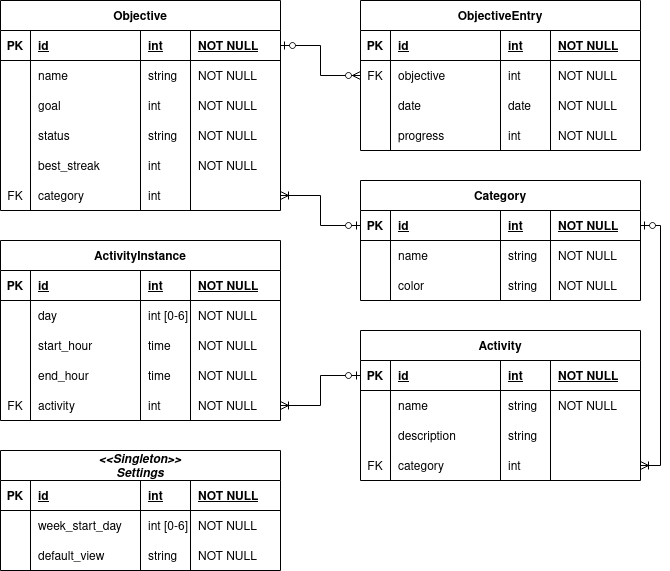
\includegraphics[scale=0.6]{img/sprint5-modelo-datos.png}
	\caption{Diagrama Entidad-Relación actualizado en el \textit{Sprint 5}}
\end{figure}


\subsubsection{Implementación}

\textbf{TFG-38}

En la aplicación del servidor, se añadió el campo correspondiente al modelo de \textbf{configuración} para guardar una vista por defecto. Se construyó un enumerado con los posibles valores, y un validador personalizado para evitar guardar valores extraños.

En el cliente, se añadió el campo de vista por defecto tanto al modelo de configuración como al contexto de la aplicación, y se actualizó el formulario de ajustes para permitir seleccionar las distintas vistas disponibles.

\medskip

\textbf{TFG-40}

Para implementar esta tarea se revisó el listado de problemas de contraste proporcionado por las herramientas de accesibilidad de Firefox, principalmente localizados en el historial de entradas de objetivos, y se ajustaron los valores necesarios para cumplir con los contrastes requeridos por el criterio de éxito 1.4.3 de las reglas \textit{WCAG 2.0} \cite{noauthor_understanding_nodate}.

\medskip

\textbf{TFG-91}

Para implementar esta tarea, fue necesario aplicar los ajustes manuales para equiparar el número del día de la semana entre TypeScript y Python elaborados con anterioridad. Se modificó la forma de construir la estructura flexbox de la vista de actividades, mostrando las columnas de los días en orden, comenzando por el día definido en el contexto global de la aplicación.

Se intentó ajustar el resto de calendarios de la aplicación, es decir, los usados en el historia de entradas de objetivos y los selectores de fecha. No obstante, la configuración de dichos componentes respondía a criterios distintos, siendo necesarias herramientas de internacionalización \cite{noauthor_diferencias_nodate}, por lo que quedaron pendientes.


\subsubsection{Otros}

Se implementaron notificaciones de éxito o fracaso de las operaciones relacionadas con la API en el cliente, utilizando la herramienta \textit{Notistack} \cite{dehnokhalaji_notistack_nodate}.

Se actualizó la documentación de la API a la la versión OpenAPI 3.0, ofreciendo una mayor expresividad a la hora de definir tipos y esquemas.


\subsubsection{Pruebas}

Se dedicó el resto de la iteración a probar exhaustivamente las funcionalidades implementadas hasta la fecha, y recoger las distintas sugerencias e ideas proporcionadas para ser planteadas en el futuro.


\subsection{Octava iteración: \textit{Sprint 6}}

\textbf{Inicio:} 21 de agosto

\textbf{Fin:} 31 de agosto

\subsubsection{Análisis}

La última iteración se destinó a evaluar el estado de la aplicación, realizar los cambios necesarios, y explorar las historias de usuario que respondían a requisitos opcionales o de muy baja prioridad pendientes.

Las historias de usuario asignadas originalmente son las siguientes:

\textbf{Sprint 6}
\begin{itemize}[leftmargin=16mm]
	\item [\textbf{TFG-13}] Como usuario, quiero poder definir objetivos con varios tipos de progreso, para poder flexibilizar mis objetivos .
	
	\item [\textbf{TFG-28}] Como usuario, quiero ver las actividades asociadas a una categoría en la vista de esa categoría para poder ver fácilmente cuáles son.
	
	\item [\textbf{TFG-35}] Como usuario, quiero poder establecer mi zona horaria para que el reloj y el progreso funcionen adecuadamente.
	
	\item [\textbf{TFG-37}] Como usuario, quiero poder seleccionar el tema de la aplicación para acomodarla a mis gustos y necesidades.
	
	\item [\textbf{TFG-81}] Como usuario, quiero poder ocultar el panel lateral para poder ver con mayor tamaño el resto de la aplicación.
\end{itemize}

Se exploró la aún pendiente funcionalidad de pausar objetivos descrita en la historia de usuario TFG-19. No obstante, las ideas que surgieron supondrían grandes cambios en la estructura de los objetivos, por lo que se exploraría en un futuro para cumplir el plazo de entrega de la forma más ajustada posible.

Con respecto a la historia TFG-28, dado que la vista de categoría es realmente un filtro sobre la vista de objetivos, se plantearon serias dudas. Introducir una lista de actividades en la vista de objetivos supondría romper la separación entre ambas partes de la aplicación, y se decidió cancelar la implementación de esta característica. Se propusieron, no obstante, futuras funcionalidades a implementar en la vista de objetivos ---y categoría---, relacionadas con el análisis de los datos registrados de forma visual.

La historia TFG-35 también fue revisada, ya que, para trabajar con ajustes manuales sobre la zona horaria, sería necesario replantear muchas de las funcionalidades implementadas, los estándares utilizados para el almacenamiento de fechas, la internacionalización de varios módulos de la aplicación, y el uso de bibliotecas externas que habría que dominar previa implementación. Al igual que la historia TFG-19, se decidió posponer su realización para ajustarse a la entrega sin afectar al trabajo ya realizado.

En cuanto a la historia de usuario TFG-37, se planteó la posibilidad de utilizar las capacidades de Material UI para definir un tema visual, y elegir entre una serie de opciones predefinidas en los ajustes de la aplicación. Además, surgió la idea de utilizar el color definido en una categoría para representar la vista de la misma. Se idearon un total de doce temas, correspondiendo con los posibles colores asignables a una categoría, utilizando colores de la paleta de \textit{Material Design}.

Por último, se descartó la historia de usuario TFG-13 debido a que no encajaba con el enfoque de la aplicación tomado.

\subsubsection{Diseño}

Al llegar a esta iteración, todas las consideraciones de diseño de la aplicación habían sido tomadas. No obstante, para añadir la elección del tema de la aplicación, fue necesario modificar el modelo de configuración para añadir el tema seleccionado.

El modelo de datos final queda representado en el siguiente diagrama:

\begin{figure}[hbt!]
	\centering
	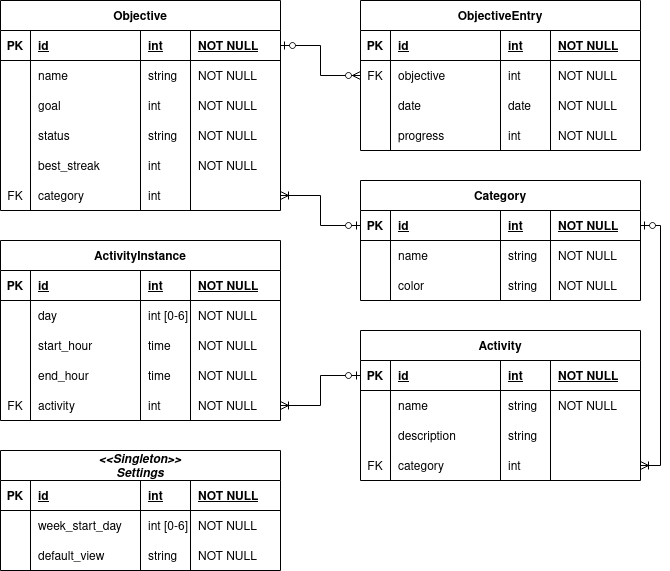
\includegraphics[scale=0.6]{img/sprint5-modelo-datos.png}
	\caption{Diagrama Entidad-Relación final}
\end{figure}

\subsubsection{Implementación}

Se implementaron los temas descritos en la historia TFG-37, se añadió el campo correspondiente en el modelo de datos y un enumerado con los distintos temas disponibles, para validar el modelo en la base de datos.

En el cliente, se añadieron los distintos temas utilizando las herramientas proporcionadas por Material UI. Se añadió el campo de tema al formulario de configuración, al modelo y al serializador. 

Para conseguir cambiar el tema por el color definido en cada categoría en la vista correspondiente, se decidió almacenar la lista de categorías en el contexto de la aplicación, ya que era necesario consultar los valores desde muchos componentes, y era la opción más cómoda, además de uno de los casos de uso del contexto en React.


\subsubsection{Pruebas}

Se realizaron pruebas exhaustivas de uso de la aplicación, además de comprobar que los tests definidos en la base de datos seguían siendo superados sin problemas.

Se concluyó que se habían alcanzado los objetivos previstos, salvo las excepciones acordadas, y el encargo había sido entregado en el plazo correspondiente.


% Capítulo: conclusiones y vías futuras
\chapter{Conclusiones y vías futuras}

\section{Conclusiones del proyecto}

La propuesta inicial de este proyecto fue la de profundizar en el uso de tecnologías web, metodologías de desarrollo y gestión de un proyecto a largo plazo
de forma directa, utilizando para ello una propuesta verosímil, como es la de una <<aplicación de gestión de horarios>>, que va tomando forma a lo largo de distintas reuniones, estudios de mercado, propuestas de requisitos, análisis de complejidad y planificación. 


\subsubsection*{Metodología de desarrollo}

Al haber trabajado previamente con metodologías ágiles, se decidió que ofrecerían el mejor marco de trabajo posible dadas las dimensiones del proyecto y las circunstancias en las que sería desarrollado, y ha probado ser una muy buena decisión. La flexibilidad de las historias de usuario ha permitido añadir y modificar funcionalidades de forma rápida y directa, y al realizarse la planificación desde el punto de vista del usuario final, ha sido sencillo identificar aquellos elementos que, o bien no tenía sentido incluir, o se propusieron inicialmente, pero quedaron descartados con el tiempo al haberse concluido que no eran relevantes.

La utilización de herramientas como \textit{Jira Software}, un tablero \textit{Kanban} o elementos de \textit{SCRUM} y \textit{eXtreme Programming} para confeccionar una metodología ágil individual fue un reto al principio, pero con algunos ajustes, como la exhaustiva planificación realizada en respuesta a un primer concepto fallido, o la decisión de no incluir fases de retrospectiva dado el carácter individual del proyecto, se ha logrado definir un marco de trabajo funcional, manteniendo el proceso iterativo y flexible de las metodologías ágiles más populares.


\subsubsection{Tecnologías utilizadas}

De forma previa a este proyecto, la experiencia en desarrollo de aplicaciones web era mínima. Se había trabajado ocasionalmente con HTML, y se realizó una página web sencilla en las prácticas de la asignatura Sistemas de Información Basados en Web, pero para realizar un proyecto con las características deseadas, era necesario aprender nuevas tecnologías, estudiar patrones de diseño, adoptar estándares utilizados y, dado que se intentaba simular un encargo profesional, realizar un estudio de herramientas populares y valoradas por empresas de desarrollo. 

La implementación de los requisitos propuestos en la aplicación desarrollada demuestra la adquisición de dichos conocimientos y el manejo de las tecnologías elegidas. A continuación se detallan los aspectos más destacables de cada una de ellas.

\textbf{Conocimientos adquiridos en materia de desarrollo \textit{back-end}}

Django ha permitido liberar mucha carga de trabajo a la hora de configurar conexiones entre la capa de datos y la de aplicación, definir una abstracción sobre el modelo, implementar relaciones entre distintas entidades y servir una API REST plenamente funcional y siguiendo estándares abiertos. No obstante, es una herramienta muy compleja, con multitud de conceptos y formas de trabajar específicas, que han entorpecido en varias ocasiones el desarrollo. No obstante, es indudable que la elección de Django como marco de trabajo para definir la capa de aplicación ha sido acertada, y ha permitido dedicar más tiempo al diseño y correcto funcionamiento de las funcionalidades específicas descritas en los requisitos.

La elección de ofrecer una documentación utilizando el estándar OpenAPI fue motivada, entre otros factores, por el uso de la herramienta Swagger UI. Sin embargo, ha evitado errores de forma temprana y permitido definir la estructura de la API desarrollada de forma mucho más clara e intuitiva, y, aunque no haya sido utilizado en este proyecto, permitiría a otros clientes consultar la estructura de la misma de forma programática.

\bigskip

\textbf{Conocimientos adquiridos en materia de desarrollo \textit{front-end}}

El uso de React como biblioteca para desarrollar la experiencia de usuario ha sido muy satisfactorio. Se trata de un proyecto acorde con la filosofía de trabajo planteada inicialmente, con un ecosistema de proyectos comunitarios amplio y una documentación sencilla pero completa.

Aunque en un principio la decisión de utilizar TypeScript se tomó con reservas, ha probado ser un acierto a lo largo de todo el desarrollo, evitando errores de forma temprana, proporcionando definiciones y aclaraciones útiles para integrar herramientas de terceros y un proceso de serialización y deserialización de datos mucho más cómodo y seguro que el posible utilizando JavaScript, entre otras ventajas. Además, no ha sido necesario dedicar un gran esfuerzo en adaptarse a TypeScript, puesto que su sistema de tipos es similar a lenguajes ya aprendidos previamente. 

Por último, la utilización de la biblioteca Material UI ha resultado realmente útil a la hora de ajustarse a los prototipos y bocetos realizados en las fases tempranas del proyecto, ofreciendo un diseño intuitivo y flexible, una gran variedad y una documentación muy completa. Ha sido fácil de adaptar al entorno de desarrollo y no ha presentado problemas de forma posterior, a diferencia de otras opciones exploradas.


\subsubsection{Aplicación desarrollada}

La aplicación cumple con los objetivos propuestos inicialmente, extraídos de un análisis de aplicaciones similares y usuarios objetivo. Si bien es cierto que los plazos inicialmente propuestos fueron incumplidos, se trataba de un planteamiento poco realista, y se evaluó la situación para solucionarlo con un nuevo calendario de trabajo, que se ha respetado de forma adecuada, y haciendo un mejor uso de las herramientas escogidas.

A la hora de elaborar el presupuesto aproximado del desarrollo, se exploraron las distintas opciones de la plataforma \textit{AWS}, lo cual ayudó a comprender el funcionamiento de la misma de cara al cliente: cómo contratar servicios en la nube, qué instancias son adecuadas para la aplicación desarrollada o qué servicio de base de datos elegir, entre muchas otras opciones.

En general, la aplicación se ajusta a los requisitos planteados. Se ha ofrecido una aplicación web desarrollada utilizando metodologías ágiles y tecnologías modernas, con una arquitectura escalable respetando la separación Modelo-Vista-Controlador y una experiencia de usuario ajustada a la propuesta realizada.


\section{Aspectos a mejorar}

\subsection*{Mejor uso de Git}

Uno de los principales aspectos a mejorar del proyecto es un mejor control de versiones. Se ha utilizado Git a lo largo de todo el proyecto, pero al consistir el equipo de un único desarrollador, se decidió no profundizar en el uso de características como ramas o integración continua proporcionada por plataformas como GitHub o GitLab.

En retrospectiva, estos cambios hubiesen mantenido las versiones del proyecto mucho mejor estructuradas, y de haberse producido algún fallo o cambio drástico, hubiese sido mucho más sencillo trabajar con él.


\subsection*{Planificación flexible, pero concreta}

Sin duda, la planificación inicial elaborada en el proyecto tiene grandes fallos a primera vista, y pese a haberse corregido, causó el retraso de la entrega del proyecto.
Una planificación más concreta, con iteraciones mejor definidas, tareas estimadas de antemano y previsión de posibles obstáculos hubiese ahorrado gran cantidad de problemas en el desarrollo del proyecto.


\subsection{Detección temprana de relaciones de dependencia entre tareas}

La tardía implementación de la barra lateral en el proyecto bloqueó multitud de tareas casi completadas, por lo que dedicar mayor tiempo en la fase de planificación a definir dependencias entre tareas y tenerlas en cuenta a la hora de distribuirlas en las iteraciones descritas hubiese sido beneficioso para el desarrollo.


\subsection*{Uso de OpenAPI 3.0 desde el principio}

Pese a ser un detalle menor, el cambio entre las versiones 2.0 y 3.0 de OpenAPI simplificó en gran medida la forma de definir la documentación de la API. Se decidió no implementarlo en un principio debido a una mayor complicación al configurar Swagger UI, pero una vez realizada la actualización, la herramienta no supuso problema alguno.


\section{Posibles modificaciones futuras}

Se han ideado posibles planes futuros en caso de que el proyecto continuase su desarrollo.

\subsection*{Implementación de las funcionalidades opcionales cubiertas en los objetivos}

Como se concluyó en la última iteración, algunas de las funcionalidades opcionales quedarían pendientes para su desarrollo en el futuro:

\begin{itemize}
	\item Posibilidad de pausar y reanudar objetivos manteniendo las rachas conseguidas
	\item Posibilidad de seleccionar la zona horaria de la aplicación
\end{itemize}


\subsubsection*{Despliegue en un entorno de producción}

El proyecto se ha ejecutado y probado utilizando los servidores de desarrollo proporcionados por Django y React. No obstante, uno de los planes previstos es 
servir la aplicación desde un entorno contratado en AWS, utilizando las instancias descritas en el presupuesto. Esto requiere preparar la aplicación para dicho entorno, así como migrar la base de datos a la instancia requerida.

Alternativamente, se podría desplegar la aplicación en un cluster de servidores locales, configurado con las herramientas y sistemas necesarios para garantizar la integridad y seguridad de la misma, a la vez que maximizar el tiempo de actividad.


\subsubsection*{Adaptación del cliente a dispositivos móviles}

Pese a que la aplicación cuenta con un diseño adaptable a distintas resoluciones, sería deseable contar con una experiencia de usuario diseñada para móviles, ya sea adaptando el cliente actual o desarrollando uno específico.


\subsubsection*{Estadísticas de cumplimiento de objetivos}

Una de las ideas propuestas en la última iteración del desarrollo es la de mostrar diversas estadísticas basadas en los datos registrados, como gráficas de cumplimiento de objetivos por mes, métricas de constancia y similares. Se mostrarían en la la vista de objetivos, junto al historial.


\subsubsection*{Modos de visualización alternativos para la vista de actividades}

La vista de actividades implementada consiste en una colección de listas de elementos que muestran las diferentes actividades definidas cada día de la semana. Se desea ofrecer la posibilidad de alternar entre este modo y otro similar a un horario, en el que las actividades aparecen en su lugar correspondiente.


\newpage

% Capítulo: bibliografía
\bibliographystyle{apalike}
\addcontentsline{toc}{chapter}{Bibliografía}
\bibliography{bibliography}







\end{document}
